%\documentclass[10pt,twocolumn]{article}
\documentclass{sig-alternate}
\usepackage{color,graphicx}
\usepackage{hhline}
\usepackage{alltt}
\usepackage{url}
\usepackage{times}
\usepackage{mathptmx}
\usepackage{xspace}
\usepackage{cite}
\usepackage{color}
\usepackage{epsfig}
\usepackage{theorem}

\usepackage{amsmath,amssymb,amsfonts}
%\usepackage{times}
\usepackage{theorem}
\usepackage{color,graphicx}
\usepackage{boxedminipage}
\usepackage{program}
\usepackage{float}
\usepackage{array}
\usepackage{multirow}
\usepackage[tight]{subfigure}
\usepackage{fancyhdr}
\usepackage{calc}
%\usepackage{bibspacing}

\theoremstyle{plain}
\setlength{\theorempostskipamount}{5pt}
\setlength{\theorempreskipamount}{5pt}
%%%%%%%%%%%%%%%%%%%%%%%%%%%%%%%%%%%%%%%%%%%%%%%%%%%%%%%%%
\newtheorem{Def}{Definition}
\newtheorem{Not}{Notation}
\newtheorem{Claim}{Claim}
\newtheorem{Theorem}{Theorem}
\newtheorem{Lem}{Lemma}
\newtheorem{Cor}{Corollary}
\newtheorem{Example}{Example}
\newtheorem{Assumption}{Assumption}
\newtheorem{Constraint}{Constraint}
%%%%%%%%%%%%%%%%%%%%%%%%%%%%%%%%%%%%%%%%%%%%%%%%%%%%%%%%%
\renewcommand{\qedsymbol}{\square}
\newcommand{\QED}{%
  \relax
  \ifvmode
  \noindent
  \else
  \unskip 
    % Remove a preceding space so only the \quad is left
  \hskip0pt plus-1fill\relax % this is like \hfilneg
  \fi
  \vrule width0pt 
      % put in a nondiscardable object to prevent the
      % \hfill from disappearing if the line breaks here
  \nobreak
  \hfill % \hfill with two l's to overpower \parfillskip
  \quad
  \qed%
}
%%%%%%%%%%%%%%%%%%%%%%%%%%%%%%%%%%%%%%%%%%%%%%%%%
\providecommand{\floor}[1]{\lfloor #1 \rfloor}
\providecommand{\ceil}[1]{\lceil #1 \rceil}
\providecommand{\abs}[1]{\lvert#1\rvert}
\providecommand{\norm}[1]{\lVert#1\rVert}
\providecommand{\dvds}[2]{#1\lvert#2}
\providecommand{\card}[1]{\lvert#1\rvert}
\providecommand{\aset}[1]{\{#1\}}
\providecommand{\lat}[1]{\langle{#1}\rangle}
\providecommand{\sig}[1]{\texttt{(#1)}}
\providecommand{\ssig}[1]{\texttt{[#1]}}
%%%%%%%%%%%%%%%%%%%%%%%%%%%%%%%%%%%%%%%%%%%%%%%%%%%%%%%%%
\providecommand{\lcm}{\emph{lcm}}
\providecommand{\gcd}{\emph{gcd}}
%%%%%%%%%%%%%%%%%%%%%%%%%%%%%%%%%%%%%%%%%%%%%%%%%%%%%%%%%
\floatstyle{ruled}
\newfloat{Algorithm}{thp}{lop}
\floatstyle{ruled}
\newfloat{Query}{thp}{lop}
%%%%%%%%%%%%%%%%%%%%%%%%%%%%%%%%%%%%%%%%%%%%%%%%%%%%%%%%%
\newcommand{\naive}{na\"{i}ve }
\newcommand{\etal}{et al.}
%%%%%%%%%%%%%%%%%%%%%%%%%%%%%%%%%%%%%%%%%%%%%%%%%%%%%%%%%%%%
\renewcommand{\ttdefault}{cmtt}
\newenvironment{myitemize}{\begin{list}{$\bullet$}{
        \setlength{\itemsep}{-5pt}
}}{ \end{list}}
%%%%%%%%%%%%%%%%%%%%%%%%%%%%%%%%%%%%%%%%%%%%%%%%%%%%%%%%%%%%
%\renewcommand{\ttdefault}{cmtt}
%\newcounter{foo}
%\newenvironment{myenumerate}{\begin{list}{\arabic{foo}.}{
%        \usecounter{foo}
%        \setlength{\itemsep}{-5pt}
%        \setlength{\itemsep}{-1pt}
%}}{ \end{list}}
%%%%%%%%%%%%%%%%%%%%%%%%%%%%%%%%%%%%%%%%%%%%%%%%%%%%%%%%%%%%
\newcounter{hours}\newcounter{minutes}
\newcommand{\printtime}{%
  \setcounter{hours}{\time/60}%
  \setcounter{minutes}{\time-\value{hours}*60}%
  \thehours:\theminutes}
%%%%%%%%%%%%%%%%%%%%%%%%%%%%%%%%%%%%%%%%%%%%%%%%%%%%%%%%%%%%
\providecommand{\LAR}{\leftarrow}
\providecommand{\RAR}{\rightarrow}
\providecommand{\DOT}{\centerdot}
\providecommand{\satisfies}{\rightarrow}
%%%%%%%%%%%%%%%%%%%%%%%%%%%%%%%%%%%%%%%%%%%%%%%%%%%%%%%%%%%%

\def\RETURN{\keyword{return}}
\def\ubar#1{\underbar{#1}}



\newcommand{\comment}{\textcolor{red}}
\newcommand{\link}[1]{{\small \url{#1}}}
\newcommand{\note}[1]{}

\def\Pitu{P2\xspace}
\def\Sys{\Pitu}
\def\sysx{\Pitu}
\def\Dlog{{\em NDlog}\xspace}
\def\link{\texttt{\#link}\xspace}
\def\bilink{\texttt{\#bilink}\xspace}
\def\dblspace{\xspace\xspace}
\def\eg{{\sc $e.g.,~$}}
\def\ie{{\sc $i.e.,~$}}
\def\Eg{{\sc $E.g.,~$}}
\def\Ie{{\sc $I.e.,~$}}
\def\manyquads{\quad\quad\quad\quad\quad\quad\quad\quad}

%\setlength{\oddsidemargin}{-0in}
%\setlength{\evensidemargin}{-0in}
%\setlength{\hoffset}{-0.25in}
%\setlength{\textwidth}{7in}
%\setlength{\topmargin}{0.1in}
%\setlength{\voffset}{-0.25in}
%\setlength{\headheight}{-0.3pt}
%\setlength{\headsep}{0pt}
%\setlength{\textheight}{9.3in}

\addtolength{\parindent}{-1mm}
\addtolength{\parskip}{-0.2mm}
%\addtolength{\belowcaptionskip}{-2mm}
%\addtolength{\abovecaptionskip}{-2mm}

\addtolength{\dblfloatsep}{-2mm}
\addtolength{\dbltextfloatsep}{-2mm}
\setlength{\columnsep}{1.45pc}
\linespread{0.943}
%\linespread{1}

% Compact itemize and enumerate. Note that they use the same counters and
% symbols as the usual itemize and enumerate environments.
\def\compactify{\itemsep=0pt \topsep=0pt \partopsep=0pt \parsep=0pt}
 \let\latexusecounter=\usecounter
 \newenvironment{CompactItemize}
   {\def\usecounter{\compactify\latexusecounter}
    \begin{itemize}}
   {\end{itemize}\let\usecounter=\latexusecounter}
 \newenvironment{CompactEnumerate}
   {\def\usecounter{\compactify\latexusecounter}
    \begin{enumerate}}
   {\end{enumerate}\let\usecounter=\latexusecounter}


\begin{document}

% SIGMOD Copyright
%\conferenceinfo{SIGMOD 2006}{June 27-29, 2006, Chicago, Illinois, USA}
%\CopyrightYear{2006}
%\crdata{1-59593-256-9/06/0006}

% Avoid SIGMOD Copyright
%\def\copyrightspace{}
\toappear{Appears in the ACM SIGMOD International Conference on Management of Data, Chicago, IL, USA, June 2006.}  


\newcommand{\dataloglabel}[1]{\mbox{\bf #1:}\hfil}
\newenvironment{datalog}
  {\begin{list}{}%
      {\it \small \renewcommand{\makelabel}{\dataloglabel}%
    \setlength{\parsep}{-2pt}%
    }%
  }%
{\end{list}}

\newcommand{\datalogspace}{\textcolor[gray]{1}{.}\hspace{0.8in}}


\renewcommand{\ttdefault}{cmtt}
\newcounter{foo1}
\newenvironment{myenumerate}{\begin{list}{\arabic{foo1}.}{
      \usecounter{foo1}
      \setlength{\itemsep}{0mm}
      \setlength{\topsep}{0mm}
      \setlength{\itemsep}{-2pt}
}}{ \end{list}}

\newenvironment{mylist}{\begin{list}{$\bullet$}
    {
      \setlength{\itemsep}{0mm}
      \setlength{\topsep}{0mm}}
    }
{\end{list}}


\newcommand{\calS}{\mathcal{S}}
\newcommand{\calD}{\mathcal{D}}
\newcommand{\eat}[1]{}



% \title{Declarative Networking with\\Distributed Recursive Query
% Processing}
\title{Declarative Networking:\\Language, Execution and Optimization}

\author{Boon Thau Loo\thanks{\scriptsize UC Berkeley authors funded
  by NSF grants 0205647, 0209108, and 0225660, and a
  gift from Microsoft.} \dblspace Tyson Condie$^*$ \dblspace Minos Garofalakis$^\dagger$\dblspace David E.\ Gay$^\dagger$\dblspace Joseph
  M.\ Hellerstein$^*$\dblspace\\Petros Maniatis$^\dagger$\dblspace Raghu Ramakrishnan$^\ddagger$\dblspace Timothy
  Roscoe$^\dagger$\dblspace Ion Stoica$^*$\\ {\small $^*$UC Berkeley, $^\dagger$Intel Research Berkeley and
  $^\ddagger$University of Wisconsin-Madison}}

\date{}

\maketitle

\begin{abstract} 
  The networking and distributed systems communities have recently
  explored a variety of new network architectures, both for
  application-level overlay networks, and as prototypes for a
  next-generation Internet architecture.  In this context, we have
  investigated {\em declarative networking}: the use of a distributed
  recursive query engine as a powerful vehicle for accelerating
  innovation in network
  architectures~\cite{declareRoute,declareOverlays,singhEurosys}. 
  Declarative networking represents a significant new application area for
  database research on recursive query processing. In this paper, we
  address fundamental database issues in this domain. First, we
  motivate and formally define the Network Datalog (\Dlog) language
  for declarative network specifications.
%   We introduce the concept of {\em link-restricted}
%   rules, which can be syntactically guaranteed to be executable via
%   single-node derivations and message passing on an underlying network
%   graph. 
  Second, we introduce and prove correct relaxed versions of the
  traditional semi-\naive query evaluation technique, to overcome fundamental
  problems of the traditional technique in an asynchronous distributed
  setting.  Third, we consider the dynamics of network state, and
  formalize the ``eventual consistency'' of our programs even when
  bursts of updates can arrive in the midst of query execution.
  Fourth, we present a number of query optimization opportunities that
  arise in the declarative networking context, including applications
  of traditional techniques as well as new optimizations. Last, we
  present evaluation results of the above ideas implemented in our
  \Sys declarative networking system, running on 100 machines over the
  Emulab network testbed.
\end{abstract}



\section{Introduction} 
\label{sec:intro} 
Although distributed programming has become an essential and commonplace task,
it remains very challenging for most developers to write correct distributed
programs. The inherent difficulties of distributed computing---concurrency,
asynchrony, and partial failure---are exacerbated by the scale at which modern
distributed systems operate.

% remind reviewers that it's a database problem. can remove if accepted! 
Much of the discussion about distributed programming today revolves around data
management systems, and the tradeoffs between transactions and loose
consistency. Programmers using distributed transactions are relieved of
consistency concerns but often face significant performance and operational
challenges~\cite{Birman2009}. By contrast, programmers who use loosely
consistent systems can expect more predictable and low-latency performance, but
must reason explicitly about program correctness over inconsistent distributed
state.

In recent years there has been increased interest in techniques to help
programmers achieve correct program behavior without requiring strongly
consistent storage. This idea has been explored in two different frameworks,
\emph{Convergent Objects} and \emph{Monotonic Logic}.

\vspace{0.5em}\noindent
\textbf{Convergent Objects}: In this approach, a programmer writes encapsulated
object classes whose public methods guarantee certain properties regarding
message reordering and/or retry. For example, Statebox is an open-source library
that merges conflicting updates to data items in a key-value store; the user of
the library need only register commutative, idempotent merge
functions~\cite{statebox}. This approach has roots in research in
databases~\cite{Farrag1989,Garcia-Molina1983,Helland2009} and
groupware~\cite{Ellis1989,Sun1998}.  Shapiro et al.\ recently proposed a model
for these approaches called \emph{Conflict-Free Replicated Data Types} (CRDTs),
which formalizes these ideas in an algebraic framework~\cite{Shapiro2011b}.

The main problem with the CRDT approach is that its guarantees of correctness
are limited to an individual replicated data value, not to application logic in
general. For example, consider a distributed algorithmic trading service that
uses a CRDT to represent a mutable set \texttt{Portfolio}. Suppose one server
$M$ reads a local version of the set containing an element \texttt{BNNA} and
constructs an expected portfolio value $v = f(\mbox{\texttt{Portfolio}})$
derived from that version. Concurrently, \texttt{BNNA} is removed from the local
version of \texttt{Portfolio} at another server $N$. The CRDT can ensure that
$M$ and $N$ will eventually agree that \texttt{BNNA} is absent from the set, but
the application state at $M$ and $N$ may remain inconsistent unless the value
$v$ at $M$ is updated to reflect the removal of \texttt{BNNA}. Although the CRDT
maintains its own invariants, the programmer still bears the burden of ensuring
the consistency semantics of the entire program.

\vspace{0.5em} \noindent
\textbf{Monotonic Logic}: In recent work, we observed that the database theory
literature on non-monotonic logic provides a promising starting point for
reasoning about distributed consistency. Intuitively, a \emph{monotonic} program
computes more information over time---it never ``retracts'' an earlier
conclusion in the face of new information. We proposed the CALM
theorem~\cite{Hellerstein2010}, which established that all monotonic programs
are eventually consistent~\cite{Ameloot2011,dedalus-pods12-tr}. Monotonicity of
a Datalog-style program is straightforward to determine conservatively from
syntax, so the CALM theorem provides the basis for a simple analysis technique
for verifying the consistency of distributed programs~\cite{Alvaro2011}. We
realized the CALM analysis as part of Bloom, a Datalog-based DSL for distributed
programming~\cite{bloom}.

The original formulation of Bloom and CALM only validated consistency for programs that compute sets of facts that grow over time (``set monotonicity''); that is, ``growth'' is defined according to set containment. As a practical matter, this is overly conservative: several common distributed programming idioms that are monotonic do not satisfy syntactic monotonicity tests for Datalog. In particular, threshold tests over monotonic aggregate values (e.g., ``$\mathrm{max}(S) > k$'') and upward-moving mutable counters are both considered to be non-monotonic by the original CALM analysis.  As a result, the initial Bloom prototype advises the programmer to guard those constructs with strong consistency methods like Paxos~\cite{Lamport1998} or Two-Phase Commit. 

\subsection{A Hybrid Approach}
% The strengths and weaknesses of these two approaches appear complementary. CRDTs provide synchronization-free consistent objects, but cannot guarantee whole-program consistency. Bloom's CALM analysis guarantees whole-program consistency but is unable to verify a number of natural coordination-free mechanisms.
In this paper, we extend our previous work to accommodate the ideas underlying CRDTs. Instead of only allowing growth according to the set containment
partial order, we allow any user-defined partial order to be used.  
We do this by providing \emph{join semi-lattices} as a programming construct.
We give a
formal definition of this construct below, but the intuition is that the programmer provides a commutative, idempotent merge function (``least upper bound'')
that takes two input values and produces an output value that is not smaller
than either of the input values (according to the user's partial order). This
generalizes Bloom (and traditional Datalog), which assumes a fixed merge
function (set union) and partial order (set containment).
% Relate user-defined merge functions to merge functions in other contexts?
% (e.g., key-value store, COPS, Piccolo)

% Explain how lattices generalize monotonic datalog
It is attractive to incorporate join semi-lattices into logic programming,  but doing so raises challenges in language design, consistency analysis and efficient execution.  In this paper, we make the following contributions:
\begin{enumerate}
% \item
%   We present \baselang, a variant of Datalog that is defined over lattices. We
%   define a model-theoretic semantics for \baselang, and show that \baselang
%   generalizes Datalog.

\item
  We introduce \lang, an extension of Bloom that supports lattices. We detail
  the builtin lattice types provided by \lang and show how developers can
  define new lattices.
  
\item 
  We provide interfaces for consistency-preserving mappings across lattices via
  \emph{morphisms} and \emph{monotonic functions}.  This is critical for \lang
  and forms a useful extension to the CRDT framework as well.

\item 
  We generalize the CALM analysis to programs that contain both lattices and
  set-oriented collections, and show how lattices can be used to prove the
  confluence of several common distributed design patterns that were regarded as
  non-monotonic in Bloom. % XXX: revisit this

\item
  For efficient execution, we show how to extend the standard Datalog semi-naive
  evaluation scheme~\cite{Balbin1987} to support both lattices and traditional
  database relations. We also describe how an existing Datalog engine can be
  extended to support lattices with relatively minor changes.

\item
  Finally, we demonstrate the usefulness of lattices with two case studies.
  First we revisit the simple e-commerce scenario presented in Alvaro et al., in
  which clients interact with a replicated shopping cart
  service~\cite{Alvaro2011}. We show how \lang can be used to make the
  ``checkout'' operation monotonic, despite the fact that it requires
  aggregating over a distributed data set.

  Second, we use \lang to implement vector clocks and causal delivery, two
  standard building blocks for distributed programming. We show how both
  algorithms can be realized as monotonic \lang programs that are concise and
  readable.
\end{enumerate}


\section{Data and Query Model}
\label{sec:queryModel}

We first provide a short review of Datalog, following the conventions
in Ramakrishnan and Ullman's survey~\cite{ramakrishnan93survey}. A 
Datalog program consists of a set of declarative {\em rules} and a
query. A Datalog {\em rule} has the form {\em p :- 
$q_{1}, q_{2}, ..., q_{n}$}., which can be read informally as
``$q_{1}$ and $q_{2}$ and $ ... $ and $q_{n}$ implies p''. $p$ is the {\em head} of the
rule, and $q_{1}, q_{2}, ..., q_{n}$ is a list of {\em literals} that
constitutes the {\em body} of the rule.  Literals are either {\em
predicates} applied to {\em fields} (variables and constants), or
function symbols applied to fields. The rules can refer to each other
in a cyclic fashion to express recursion. The order in which the rules
are presented in a program is semantically immaterial.  The commas
separating the predicates in a rule are logical conjuncts ({\em AND});
the order in which predicates appear in a rule body also has no
semantic significance (though implementations typically employ a
left-to-right execution strategy). The query
specifies the output of interest. 

The predicates in the body and head of Datalog rules are relations,
and we will refer to them interchangeably as predicates, relations, or
tables.  Each relation has a {\em primary key}, which consists of a
set of fields that uniquely identifies each tuple within the
relation. We allow the primary key to be specified for stored
(``extensional'') relations; in the absence of other information, the
primary key is the full set of attributes in the relation. 
%RR If you decide to remove the stuff on keys, perhaps you should
%drop the underlining convention below \ldots
%In our schema
%definitions, we \underline{underline} the primary key attributes of a
%table (unless the primary key is the full set of attributes).    
%\footnote{If
%  the primary key is not the full set of attributes, there can be multiple tuples generated with the same primary
%  key. In this case, the results set contains one of the derivations,
%  depending on the evaluation strategy and execution run.}. 

The names of predicates, function symbols
and constants begin with a lower-case letter,
while variable names begin with an upper-case letter.  Most
implementations of Datalog enhance it with a limited set of function
calls (which start with {\em ``f\_''} in our syntax), including
boolean predicates, arithmetic computations and simple list
manipulation (\eg the $f\_concatPath$ function in our first
example). Aggregate constructs are represented as functions with field
variables within angle brackets ($<>$). For most of our discussion, we
will not consider negated predicates; we will return to the topic of
negation as part of our future work (Section~\ref{sec:futurework}).

As an example, the following program computes the shortest paths between
all pairs of nodes in a graph. The program has four rules (which for
convenience we label R1-R4), and takes as input a stored
(``extensional'') relation $link(src, dst, cost)$.  R1 and R2 are used
to derive ``paths'' in the graph, represented as tuples in the
derived (``intensional'') relation $path(src, dst, nextHop, pathVector, \ldots)$.  The $src$ and
$dst$ fields represent the endpoints of the path; the $pathVector$ is
a string encoding the full path. We discuss $nextHop$ later. Given the
$path$ relation, Rule R4
computes the shortest paths as the derived relation
$shortestPath(src, dst, pathVector, cost)$. R3
derives the relation $spCost(src, dst, mincost)$ that
computes the minimum cost for each (src,dst) group for all input paths.
The rule {\em Query} specifies shortestPath tuples as the result
tuples. R2 is a {\em linear} rule, since there is only one
recursive literal in the body. Rules with more than one recursive literal
in the body are {\em non-linear}.

%In this example, {\em S}, {\em Z}, {\em D}, {\em C} and {\em P}
%abbreviate the {\em source}, {\em nextHop}, {\em destination}, {\em
%cost} and {\em pathVector} fields respectively for both the link and
%path tuples.    

\vspace{2pt} {\small
\noindent{\bf R1: } path(S,D,D,P,C) :- link(S,D,C), P = $f\_concatPath$(link(S,D,C), nil). \\
{\bf R2: } path(S,D,Z,P,C) :-
  link(S,Z,C$_{1}$), path(Z,D,Z$_{2}$,P$_{2}$,C$_{2}$),\\
\datalogspace C = C$_{1}$ + C$_{2}$, P = $f\_concatPath$(link(S,Z,C$_{1}$),P$_{2}$).\\
{\bf R3: } spCost(S,D,min$<$C$>$) :- path(S,D,Z,P,C).\\
{\bf R4: } shortestPath(S,D,P,C) :- spCost(S,D,C), path(S,D,Z,P,C).\\
{\bf Query: } shortestPath(S,D,P,C).
}
\vspace{2pt}

Rule R1 produces one-hop paths from existing link tuples, and Rule R2
recursively produces path tuples of increasing cost by matching the
destination fields of existing links to the source fields of previously
computed paths. The matching is expressed using the repeated ``Z'' variable in
$link(S,Z,C_{1})$ and $path(Z,D,Z_{2},P_{2},C_{2})$ of rule
R2. Intuitively, rule R2 says that if there is a link from node {\em S}
to node {\em Z}, and there is a path from node {\em Z} to node {\em D},
then there is a path from node {\em S} to node {\em D} via {\em Z}. In
the presence of path cycles, the query never 
terminates, as R1 and R2 will generate paths of ever increasing
lengths. However, this can be fixed with a well-known query rewrite 
(Section~\ref{subsec:aggregateSelections}) when costs are positive.% $\gt$ 0.  

%The query does not impose any restriction on either source or
%destination as both {\em S} and {\em D} are unbound
%variables. Hence, the query computes the {\em full transitive
%closure} consisting of the paths between all pairs of reachable
%nodes. If the query is only interested in the paths from a given
%node {\em b} to every other node in the network, the query would be
%$path({\bf b},D,P,C)$, with the source field bound to
%constant {\em b}.

%R3 and
%R4 together are then used to compute the shortest paths from the
%computed paths. 

\subsection{Network Datalog}

In this section, we introduce the data and query model that we propose
for declarative networking. The language we present is {\em Network
  Datalog} (\Dlog), a restricted variant of traditional Datalog intended
to be computed in distributed fashion on physical network graphs.  In
describing our model, we use the \Dlog query shown in
Figure~\ref{shortestPath}, which performs distributed computation of
shortest paths.


\begin{figure}[ht]
\begin{boxedminipage}{3.2in}
{\small
\noindent{\bf SP1: } path({\bf @S},@D,@D,P,C) :- \link({\bf @S},@D,C), \\
\datalogspace P = $f\_concatPath$(link({\bf @S},@D,C), nil). \\
{\bf SP2: } path({\bf @S},@D,@Z,P,C) :-
  \link({\bf @S},@Z,C$_{1}$), \\
\datalogspace path({\bf @Z},@D,@Z$_{2}$,P$_{2}$,C$_{2}$), C = C$_{1}$ +
C$_{2}$, \\
\datalogspace P = $f\_concatPath$(link({\bf @S},@Z,C$_{1}$),P$_{2}$).\\ 
{\bf SP3: } spCost({\bf @S},@D,min$<$C$>$) :- path({\bf @S},@D,@Z,P,C).\\
{\bf SP4: } shortestPath({\bf @S},@D,P,C) :-
spCost({\bf @S},@D,C),\\
\datalogspace path({\bf @S},@D,@Z,P,C).\\
{\bf Query: } shortestPath({\bf @S},@D,P,C).
}
\end{boxedminipage}
\small{\caption{\label{shortestPath}\emph{\small Shortest-Path
      Query in \Dlog}.}}
\end{figure}

One of the novelties of our setting, from a database perspective, is
that data is distributed and relations may be partitioned across
sites.  To ease the generation of efficient query plans in such a
system, \Dlog gives the query writer {\em explicit} control on data
placement and movement. Specifically, \Dlog uses a special data type,
{\em address}, to specify a network location.  Names of address
variables and constants are prepended with ``@''.  More formally, we
have the following definition:

\begin{Def}{\em A {\em location specifier} is an attribute of type
    address in a predicate that indicates the network storage
    location of each tuple.}
\end{Def}

As a matter of notation, we require the location specifier to be the
first field in all predicates, and we highlight it in {\bf bold} for
clarity. For example, the location specifier of $link$({\bf @S},@D,C) is {\bf @S}.

Another novelty of our setting is that we assume a network graph that
is not fully connected, \ie a node can communicate {\em directly}
with only a subset of nodes in the system.  This allows us to model
the physical connectivity of a typical autonomous system in the
Internet, where each node is connected to relatively few other nodes.
In contrast, both traditional parallel query processors and more
recent distributed query engines, such as PIER~\cite{pierCidr}, assume a
fully connected network graph, where messages can be sent directly
from any node to any other node in the system.  Parallel systems
achieve this by engineering (and provisioning) the interconnection
network, while PIER uses overlay routing to connect any two nodes.

%Our network setting is different, since the goal of networking is to
%{\em provide} full end-to-end connectivity rather than assuming it
%ahead of time. Consequently, we assume physical connectivity is
%incomplete (the normal case in a link-based network), and impose the
%constraint that messages (e.g., tuples participating in distributed
%joins) can only be exchanged between two nodes that are connected by a
%link.

To express the constraint that a node can send data only to another node with which it is
physically connected, we introduce the concept of {\em link relation},
which is defined as follows:

%Again, we want to expose this in the query language to facilitate the
%specification of messaging in the network graph.  Hence we introduce
%the following notion:

\begin{Def}{\em A {\em link relation} is a stored (``extensional'')
     relation \\$link(@src, @dst, ...)$ representing the connectivity
     information of the network being queried.}\end{Def}

%Links are defined
%using the following DDL: \texttt{linktbl
%  <tblname>(@S,@D [,<othercols>])}. 
The first two fields of each link table entry contain the source and
destination addresses of a network link respectively, followed by an
arbitrary number of other fields (typically metrics) describing the
link.  In this paper, we constrain all links to be
bidirectional, \ie if there is
a network edge from a node to its neighbor, the reverse must be true\footnote{In practice, some networks may not have
symmetric links.  Our framework can be extended to handle this, but
generalizing the discussion in that manner complicates our
presentation and is out of the scope of this paper.}.
In all our example queries, we utilize only one link table. In
practice, there can be multiple such tables used by different rules.
% , but to simplify our
% exposition we focus on a single link table in this paper.  We denote link relations
% with the syntax \link.  

Given that we will be executing queries across network links, it is useful to identify queries that do not require communication:
\begin{Def}{\em {\em Local rules} are rules that have the same
	location specifier in each predicate, including the
	head.}\end{Def}

%\begin{Def}{\em {\em Local body rules} are rules that have the same
%	location specifier in each body predicates. }\end{Def}

Local rules can be executed without any distributed logic.  Rules SP1,
  SP3 and SP4 are local. SP2 is a non-local rule since the
  $link$ and $path$ body predicates are stored at different
  locations. 

In \Dlog, the evaluation of a rule must depend only on communication
along the physical links. To this end, we introduce the following:
\begin{Def}{\em A {\em link literal} is a link relation that appears
in the body of a rule prepended with the ``\#'' symbol.}
\end{Def}
Given the preceding definitions, we are ready to define a simple
syntactic constraint on the rules to ensure that communication takes
place only along the physical links:

\begin{Def}\label{def:topRestricted} {\em A {\em link-restricted} rule
    is either a local rule, or a rule with the following properties:
\begin{mylist}
\item There is exactly one link literal in the body
\item All other literals (including the
      head predicate) have their
  location specifier set to either the first (source) or second
  (destination) field of the link literal. 
\end{mylist}}
\end{Def}

This syntactic constraint precisely captures the requirement that we
be able to operate
directly on a network whose link connectivity is not a full mesh.
Further, as we demonstrate in Section~\ref{sec:queryPro}, link-restriction
also guarantees that all programs with only link-restricted
rules can be rewritten into a canonical form where every rule body can be
evaluated on a single node. In addition, all communication for each
rewritten rule only involves sending messages along links. The
following is an example of a link-restricted rule:\\
\vspace{2pt}
{\small 
\noindent p({\bf @D},...) :- \link({\bf @S},@D,...),p$_{1}$({\bf
  @S},...),p$_{2}$({\bf @S},...), ..., p$_{n}$({\bf @S},...).
}
\vspace{2pt}

The rule body of this example is executed at @S and the resulting $p$
tuples are sent to @D, preserving the communication constraints along
links. Note that this example's body predicates all have the same
location specifier: @S, the source of the link. In contrast, rule SP2
of Figure~\ref{shortestPath} is link-restricted but has some relations whose location
specifier is the source, and others whose location specifier is the
destination; this needs to be rewritten as described in Section~\ref{sec:queryPro}. 
%A query rewrite technique described in
%Section~\ref{sec:queryPro} transforms such rules to ensure all body
%predicates are at the same location; we will apply this rewrite to all
%eligible rules to simplify our execution.


%In practice, there can be multiple topology tables used
%concurrently within a single message rule. One example is in specifying
%the Chord DHT~\cite{chord}, which requires three topology tables
%($finger$, $successor$ and $predecessor$) that can be used concurrently
%within a single rule. We do not address the use of multiple topology
%tables within a single rule in this paper.

Given these preliminaries, we are now ready to present our language \Dlog:

\begin{Def}{\em A Network Datalog (\Dlog) program is a Datalog program that satisfies
    the following syntactic constraints:
\begin{myenumerate}
\item {\bf Location specificity:} Each predicate has a location
  specifier as its first attribute 
\item {\bf Address type safety:} A variable that appears once in a
  rule as an address type must not appear elsewhere in the rule
  as a non-address type.
\item {\bf Stored link relations:} Link relations never appear in the head of a rule with a
  non-empty body (\ie they are stored, not derived).
\item {\bf Link-restriction:} Any non-local rules in the program are
  link-restricted by some link relation.
\end{myenumerate}
}
\end{Def}
Since \Dlog is a subset of Datalog, the semantics of a valid \Dlog
program are exactly those of Datalog.

\subsection{Shortest Path Example}
\label{sec:queryExec}
To illustrate \Dlog, we step through an execution of the {\em
shortest-path} query above to illustrate derivation and communication
of tuples as the query is computed. We make use of the example network
in Figure~\ref{SP example}.  Our discussion is necessarily informal
since we have not yet presented our distributed implementation
strategies; in the next section, we show in greater detail the steps
required to generate the execution plan.  Here, we focus on a
high-level understanding of the data movement in the network during
query processing.

%Here,
%  we also assume that there are no updates to the network during query
%  execution, and relax this assumption in later sections.

\begin{figure}[ht]
\centering
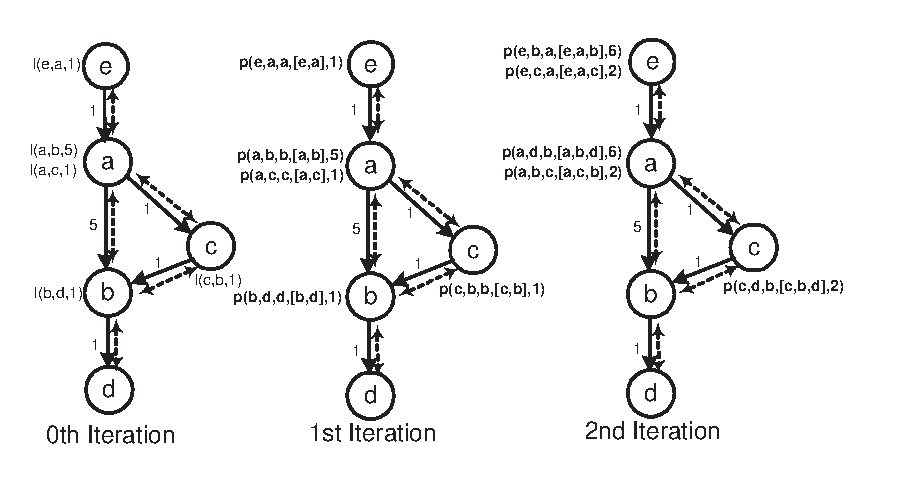
\epsfig{file=images/example.eps, width=3.5in}
\caption{\label{SP example}\emph{\small Nodes in the
    network are running the shortest-path query. We only show newly
    derived tuples at each iteration. For
    simplicity, we show only the derived paths along the
    solid lines even though the network connectivity is bidirectional (dashed lines).}}
\end{figure}                                              

We will describe communication in {\em iterations}, where at each
iteration, each network node generates $paths$ of increasing hop count, and then
propagates these paths to neighbor nodes along links. In the $1^{st}$
iteration, all nodes initialize their local path tables to 1-hop
paths using SP1. In the $2^{nd}$ iteration, using SP2, each node takes the input
paths generated in the previous iteration, and computes 2-hop paths,
which are then propagated to its neighbors. For example, $path({\bf
  a},d,b,[a,b,d],6)$ is generated at node {\em b} using
$path(b,d,d,$ $[b,d],1)$ from the $1^{st}$ iteration, and propagated to node
{\em a}. In addition to storing the entire path vector, each $path$
tuple also contains the {\em nextHop} attribute, which indicates for each path the next hop to
route the message in the network. In fact, many network protocols
propagate only the {\em nextHop} and avoid sending the entire path vector.

As paths are being computed, the shortest paths are also
incrementally computed. For example, node $a$ computes $path({\bf
  a},b,b,[a,b],5)$ using rule SP1, and then sets its shortest path to
$shortestPath({\bf a},b,$ $[a,b],5)$ using rule SP4. In the next iteration, node $a$
receives $path({\bf a},b,c,$ $[a,c,b],2)$ from node $c$ which has lower cost
compared to the previous shortest cost of 5, and hence a new $shortestPath({\bf a},b,[a,b],2)$ replaces the previous value.

%In the distributed implementation, the use of an optimization (described in Section~\ref{subsec:aggregateSelections})
%requires each node to only propagate its current shortest path to its
%neighbor node. In that case, each node only needs to maintain the
%current shortest path to every destination reported by each
%neighbor. 
%In this case, the primary key for $paths$ is
%(src,dst,nextHop).  



%This iteration is akin to
%that used in {\em semi-\naive}~\cite{semi, semi1} fixpoint evaluation techniques in traditional Datalog
%evaluation. In practice, query execution is fully asynchronous, tuples for the next round can be generated as soon as
%tuples from the previous round are computed. We will revisit this model
%of execution in later sections.




\subsection{Expressiveness}
\label{subsec:shortestPath}

In previous work~\cite{declareRoute} we argued that executing a shortest path
distributed 
Datalog query closely resembles the distributed computation of the well-known
path vector~\cite{ee122text} protocol.  In proposals for
declarative networks~\cite{declareRoute,declareOverlays}, Datalog-like programs were used
for a variety of networking tasks, including
standard routing protocols such as {\em distance
  vector}~\cite{ee122text} and {\em dynamic source
  routing}~\cite{dsr}, and more complex networks such as multicast trees
and the Chord network~\cite{chord}.  We note that \Dlog is
flexible enough for expressing most of these programs efficiently, and provides the advantages of having clear
semantics as described above (something that is not available in the
original language for \Sys described in~\cite{declareOverlays}) and a clearly defined
link-restricted implementation as described below.

%The {\em shortest-path} query is a variant of
%transitive closure computation. With minor variations, we can specify well-known
%routing protocols performing transitive closure computations. These
%include {\em distance vector}~\cite{ee122text}, {\em
%  dynamic source routing}~\cite{dsr}, best-k paths, paths with quality
%of service constraints, etc.

%Instead of computing the shortest path, by modifying
%the ``+'' and ``min'' aggregate, we can compute other types of shortest
%paths, such as the most reliable or the three least bottleneck
%paths. 
%We provide an example below that allows one to incorporate {\em
%  policy} restrictions easily on the computed shortest paths:

%\vspace{2pt}
%{\small
%\noindent{{\bf \#include(SP1,SP3,SP4)}} \\
%{\bf PR2: } path({\bf @S},@Z,@D,P,C) :-
%  \link({\bf @S},@Z,C$_{1}$), \\
%\datalogspace path({\bf @Z},@Z,$_{2}$,@D,P$_{2}$,C$_{2}$),\\
%\datalogspace excludeNode({\bf @Z},@W), C = C$_{1}$ + C$_{2}$, \\
%\datalogspace P =
%$f\_concatPath$(\link({\bf @S},@Z,C$_{1}$),P$_{2}$).\\
%{\bf Query: } shortestPath({\bf @S},@D,P,C).
%}
%\vspace{2pt}

%In this query, we introduce an additional table {\em excludeNode},
%where $excludeNode({\bf S},W)$ is a tuple that
%represents the fact that node {\em S} does not carry any traffic for
%node {\em W}. This $excludeNode$ is considered an optional predicate and
%is stored at the same location as $path$.

%To show that the restrictions do not constrain us to solely transitive closure
%computations, we present the following program below that implements the
%link flooding component of the {\em link-state}~\cite{ee122text} protocol: 

%\vspace{2pt}
%{\small
%\noindent{{\bf LS1: } flood\link({\bf @D},@S,@S,@D,C) :-
%  \link({\bf @S},@D,C)} \\
%{\bf LS2: } flood\link({\bf @M},@N,@S,@D,C) :- \link({\bf @N},@M,C$_{1}$),\\
%\datalogspace flood\link({\bf @N},@W,@S,@D,C), @M $\ne$ @W. \\
%{\bf Query: } flood\link({\bf @M},@N,@S,@D,C)
%}
%\vspace{2pt}

%flood\link({\bf @M},@N,S,D,C) is a message predicate, and
%each is tuple storing information
%about {\em \link(S,D,C)}. This tuple is flooded in the network starting
%from source node {\em S}. During the flooding process, node @M is the
%current node it is flooded to, while node @N is the node that forwarded
%this tuple to node {\em M}.  Rule LS1 generates a $floodlink$ tuple for every
%link at each node. Rule LS2 states that each node {\em N} that receives
%a $floodlink$ tuple recursively forwards the tuple to all neighbors {\em M}
%except the node {\em W} that it received the tuple from


%\subsection{Incremental Negation Evaluation}
%Negation has to stratified and computed locally. 



%\subsection{Query Convergence}

%In a static network, the query for computing all-pairs shortest paths converges in the same time
%as the diameter (in hops) of the network. However, the presence of cycles can lead
%to infinite messages. This is preventable if there is a mechanism of
%``bounding'' the recursion. Typically, this is done by not permitting
%path cycles, or enforcing bounds on the cost arguments of messages. For the latter, we have
%to enforce that all functions used in link
%structure recursion to derived tuples have cost arguments that are 
%monotonically increasing/decreasing, and queries are on bounds of these
%cost arguments or min/max aggregates. Aggregates provide a bound with
%the use of aggregate selections
%optimizations in Section~\ref{sec:queryOpt}. 


%One thing to note is that while the final query
%results for shortestPath is the same for the same input network, the intermediate paths
%generated may differ based on network dynamics and reordering of
%messages (affects how pruning is done). For example, if node a receives
%$path(a,b,c,[a,c,b],2)$ before $path(a,b,b,[a,b],5)$, then
%$path(e,b,a,[e,a,b],6)$ would not be generated due to aggregate
%selections. However, in either case, this does not affect the final
%$shortestPath(e,b,[e,c,b],2)$ being computed.




%We are not restricted to generalized transitive closure
%computations. For example, link state:%

%\vspace{2pt}
%{\small
%\noindent{{\bf LS1: } flood\link(@S},@S,@D,C,@S) :- \link(@S},@D,C)} \\
%{\bf LS2: } flood\link(@M},@S,@D,C,@N) :- \link(@N},@M,C$_{1}$),\\
%\datalogspace flood\link(@N},@S,@D,C,@W), M $\ne$ W. \\
%{\bf Query: } flood\link(@M},@S,@D,C,@N)
%}
%\vspace{2pt}



\section{Execution Plan Generation}
\label{sec:queryPro}

Having illustrated the intended execution of an example program, we
now describe the steps required to automatically generate an execution plan from a
\Dlog program. We first focus on generating
an execution plan in a centralized implementation, before extending
the techniques to the network scenario.

\subsection{Centralized Plan Generation}
\label{sec:semiNaive}

In generating the centralized plan, we utilize the well-known {\em
  semi-\naive fixpoint}~\cite{semi,semi1} evaluation mechanism that
ensures no redundant evaluations. As a quick review, in semi-\naive (SN) evaluation, input
  tuples computed in the previous iteration of a recursive rule
  execution are used as input in the current iteration to compute
  new tuples. Any new tuples that are generated for the first time in the current
  iteration are then used as input to the next iteration. This is repeated until a
  fixpoint is achieved (\ie no new tuples are produced).

The semi-\naive rewritten rule for rule SP2 is shown below:

\vspace{2pt}
{\small
\noindent{\bf SP2-1: } $\triangle$path$^{new}$({\bf @S},@D,@Z,P,C) :- \link({{\bf @S},@Z},C$_{1}$),\\
\datalogspace
$\triangle$path$^{old}$({\bf @Z},@D,@Z$_{2}$,P$_{2}$,C$_{2}$), C = C$_{1}$ + C$_{2}$, \\                              
\datalogspace P =
$f\_concatPath$(link({{\bf @S},@Z},C$_{1}$),P$_{2}$).\\ 
}

\vspace{2pt}


%SP2-1* takes as input paths ($\triangle$path$^{old}$) computed in the previous
%invocation of the rule (known as an {\em iteration}), and use that to
%compute new paths ($\triangle$path$^{new}$). 


%Since links can also be modified during query execution, we need a
%similar rewrite for links (SP2-2). 

%{\small
%\noindent{\bf SP2-2: } $\triangle$path$^{new}$({\bf @S},@Z,@D,P,C) :-
%$\triangle$link({{\bf @Z},@S},C$_{1}$),\\
%\datalogspace path({\bf @Z},@D,@N,P$_{2}$,C$_{2}$), C = C$_{1}$ + C$_{2}$, \\                              
%\datalogspace P = $f\_concatPath$(linkD({\bf @Z},@S,C$_{1}$),P$_{2}$).\\ 
%}


\begin{figure*}[ht]
\centering
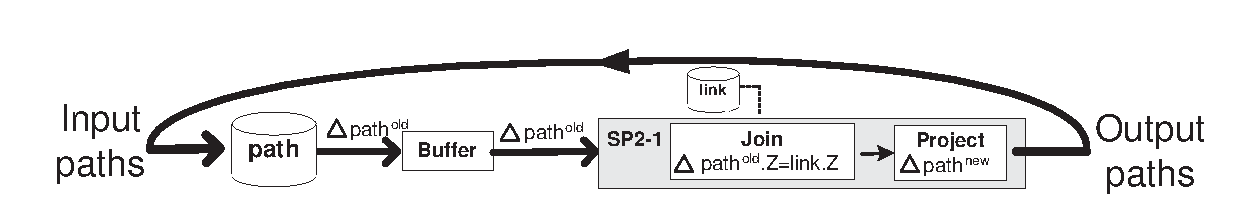
\epsfig{file=images/dataflow.eps, width=5in}
\caption{\label{Dataflow}\emph{\small Rule strand for rule SP2-1 in
    \Sys. Output paths that are generated from the strand are ``wrapped
    back'' as input into the same strand. }}
\end{figure*}                                        

Figure~\ref{Dataflow} shows the dataflow realization for rule SP2-1
using the conventions of \Sys. We will briefly explain how the semi-\naive evaluation is
achieved here. Each semi-\naive rule is implemented as a {\em rule strand}. Each strand
consists of a number of relational operators. The example strand
receives new $\triangle$$path^{old}$ tuples generated in the previous
iteration to generate new paths ($\triangle$$path^{new}$) which are
then inserted into the $path$ table (with duplicate elimination) for
further processing in the next iteration. 

In Algorithm~\ref{alg:sn}, we show the pseudocode for a centralized
\Sys implementation of multiple semi-\naive
rule strands where each rule has the form $\triangle$p$^{new}_{j}$ :-
$p^{old}_{1}$,..., $p^{old}_{k-1}$,$\triangle$p$^{old}_{k}$,$p_{k+1}$,...,$p_{n},b_{1},
b_{2},...,b_{m}$;\footnote{These rules are logically equivalent to rules
  of the form $\triangle$p$^{new}_{j}$ :- $p_{1},p_{2}$,...,$p_{k-1}$,$\triangle$p$^{old}_{k}$,$p_{k+1}$,...,$p_{n},b_{1},b_{2},...,b_{m}$,
  and have the advantage of avoiding redundant inferences within each iteration.}
\\$p_{1},...,p_{n}$ are recursive predicates and $b_{1},...b_{m}$ are base
predicates. $\triangle$p$^{old}_{k}$ refers to $p_{k}$ tuples generated
for the first time in the previous iteration. $p^{old}_{k}$
refers to all $p_{k}$ tuples generated before the previous iteration.

%|\quad | \triangle 
\vspace{2pt}
\begin{Algorithm}[ht]
  \begin{programbox}
%    |Initialize all | p_{i} | and | \triangle p^{new}_{i} to | null |
    \WHILE \exists B_{k}.size > 0
     \forall B_{k} | where | B_{k}.size > 0, \triangle p^{old}_{k} \leftarrow B_{k}.flush()
	|execute all rule strands | 	
	\FOREACH | recursive predicate | p_{j} 
	  p^{old}_{j} \leftarrow p^{old}_{j} \union \triangle p^{old}_{j}
	  B_{j} \leftarrow \triangle p^{new}_{j} - p^{old}_{j}
	  p_{j} \leftarrow p^{old}_{j} \union B_{j}
	  \triangle p^{new}_{j} \leftarrow \emptyset
%	\END
%    \END	      
\end{programbox}
\caption{Semi-\naive (SN) Evaluation in \Sys}
\label{alg:sn}
\end{Algorithm}
%end{boxedminipage}
\vspace{2pt}

In the algorithm, $B_{k}$ denotes the buffer for $p_{k}$ tuples
generated in the previous iteration
($\triangle$$p^{old}_{k}$). Initially, $p_{k}$, $p^{old}_{k}$, $\triangle$$p^{old}_{k}$ and
$\triangle$$p^{new}_{k}$ are empty. As a base case, we
execute all the rules to generate the initial $p_{k}$ tuples, which
are inserted into the corresponding $B_{k}$ buffers.  Each subsequent
iteration of the while loop consists of flushing all
existing $\triangle$$p^{old}_{k}$ tuples from $B_{k}$ and executing all
rule strands to generate $\triangle$$p^{new}_{j}$ tuples, which are used
to update $p^{old}_{j}$, $B_{j}$ and $p_{j}$ accordingly. Note that only new $p_{j}$ tuples
generated in the current iteration are inserted into $B_{j}$ for use in
the next iteration. Fixpoint is reached when all buffers are empty.
 
\subsection{Distributed Plan Generation}
\label{subsec:ruleLocalization}

In the distributed implementation of the {\em shortest-path} query,
non-local rules whose body predicates have different location
specifiers cannot be executed at a single node, since the tuples that
must be joined are situated at different nodes in the network. A {\em
  rule localization} rewrite step ensures that all tuples to be joined
are at the same node. This
allows a rule body to be locally computable.

%This step requires
%determining a distributed join ordering for predicates at different
%locations. 


\begin{figure}[ht]
\centering
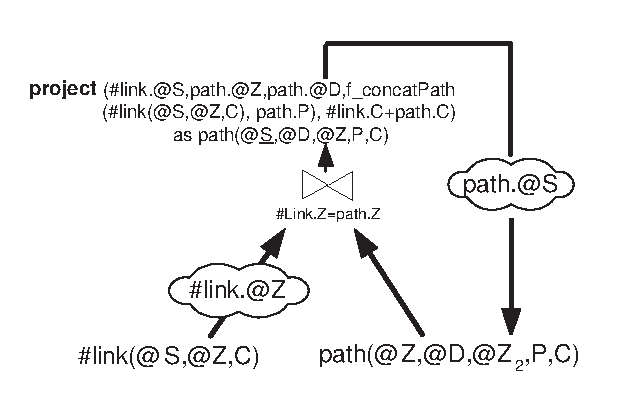
\includegraphics[width=2.5in]{images/reachable.eps}
\caption{\label{Right Reachable}\emph{\small Logical Query Plan for rule SP2 from Section~\ref{sec:queryModel}.}}
\end{figure}                                              

Consider rule SP2 from Section~\ref{sec:queryModel}
where the link and path predicates have different location specifiers. These two
predicates are joined by a common ``@Z'' address
field. Figure~\ref{Right Reachable} shows the corresponding logical
query plan depicting the distributed join. The clouds represent an
``exchange''-like operator~\cite{volcano} that forwards tuples from one
network node to another; clouds are labeled with the link attribute that
determines the tuple's recipient. The
first cloud (\link.@Z) sends link tuples to the neighbor nodes indicated by their
destination address fields, %in order 
to join with matching path
tuples stored by their source address fields. The second cloud
($path.@S$) transmits for further processing new path tuples computed
from the join, setting the recipient according to the source address field.

Based on the above distributed join, rule SP2 can be rewritten into
the following two rules. Note that all
predicates in the body of SP2a have the same location specifiers;
the same is true of SP2b.


%\begin{figure}[ht]
%\begin{boxedminipage}{3.5in}
\vspace{2pt} 
{\small
\noindent{\bf SP2a: } linkD({\bf @Z},@S,C) :- \link({\bf @S},@Z,C).\\
{\bf SP2b: } path({\bf @S},@D,@Z,P,C) :- \link({\bf @Z},@S,C$_{3}$),linkD({\bf @Z},@S,C$_{1}$), \\
\datalogspace path({\bf @Z},@D,@Z$_{2}$,P$_{2}$,C$_{2}$),\\
\datalogspace C = C$_{1}$ + C$_{2}$, \\                              
\datalogspace P =
$f\_concatPath$(linkD({\bf @Z},@S,C$_{1}$),P$_{2}$).}
\vspace{2pt} 
%\end{boxedminipage}
%\small{\caption{\label{shortestPathLocal}\emph{\small Localized Rewrite for
%      rule SP2}}}
%\end{figure}

%{\bf FIXME: insert link restricted EXCHANGE~\cite{volcano} discussion}

%Rules SP2a and SP2b have the body predicates all at the
%same location.  
%In order to join matching link tuples and path
%tuples by the ``@Z'' field, link tuples are shipped by their destination
%addresses (as the $linkD$ message predicate) using rule SP2a. Rule SP2b then performs a join of the
%arriving linkD and path tuples. 

\begin{figure*}[ht]
\centering
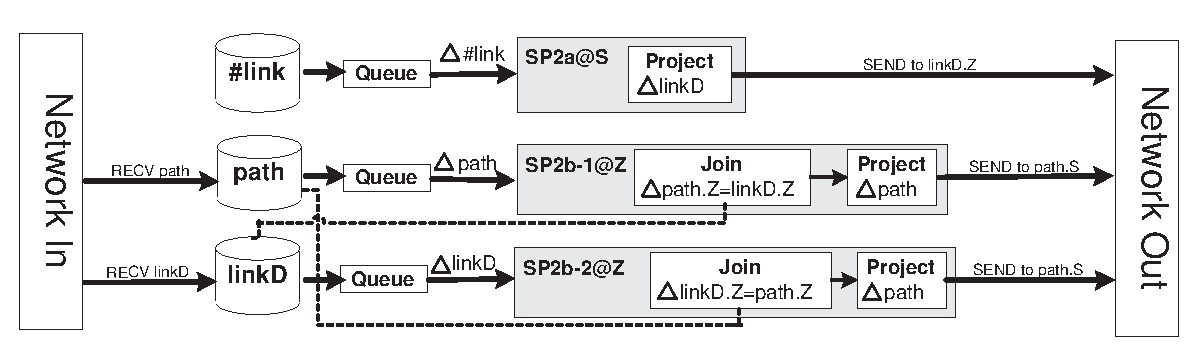
\epsfig{file=images/dataflow1.eps, width=5in}
\caption{\label{Dataflow1}\emph{\small Rule strands for the distributed
    version of SP2 after localization in \Sys.}}
\end{figure*}                                        

The rewrite is achievable because the $link$ and $path$ predicates,
although at different locations, share a common join address field. 
% Based
% on Definition~\ref{def:topRestricted}, we note that all
% link-restricted rules are localizable. 
In Algorithm~\ref{alg:ruleLocal}, we summarize the general rewrite
technique for an input set of link-restricted rules R. In the
pseudocode, for simplicity, we assume that the location specifiers of all the body
predicates are sorted (@S followed by @D); this can be done as a
preprocessing step. The algorithm as presented here assumes that all links are
bidirectional, and may add a \link(@D,@S) to a rewritten rule to
allow for backward propagation of messages.

\vspace{2pt}
{\scriptsize
\begin{Algorithm}[ht]
  \begin{programbox}
    \PROC |RuleLocalization| (R)
     \WHILE \exists | rule r |\in R|: |h(@L,...) :- |\link(@S,@D,...),|
     |\manyquads p|_{1}|(@S,..),..,p|_{i}|(@S,...),|
     |\manyquads p|_{i+1}|(@D,...),..,p|_{n}|(@D,..)| 
%     |\manyquads | \wedge | (| @L=@S | | \vee | | @L=@D )
            R.remove(r)	   
	    R.add(hS(@S,@D,..) :- |\link(@S,@D,..),..,p|_{i}|(@S,..).)|
	    R.add(hD(@D,@S,..) :- hS(@S,@D,..).)
	    \IF @L=@D 
	    \THEN R.add(|h(@D,..) :- hD(@D,@S,..),|
            |\manyquads p|_{i+1}|(@D,..),..,p|_{n}|(@D,..).|)
	    \ELSE R.add(|h(@S,..) :- \link(@D,@S),hD(@D,@S..),|
               |\manyquads p|_{i+1}|(@D,..),..,p|_{n}|(@D,..).|) 
%	       \IF \link.bidirectional
%	       | |\ELSE
%	       error(``illegal rule'')	       
%	       \FI
%            \FI
%     \END
%    \END      
\end{programbox}
\caption{Rule Localization Rewrite}
\label{alg:ruleLocal}
\end{Algorithm}
}
\vspace{2pt}

\begin{Claim}\label{claim:ruleLocal} Every link-restricted \Dlog program, when rewritten using
  Algorithm~\ref{alg:ruleLocal}, produces an equivalent program where
  the following holds:
\begin{CompactEnumerate}
\item The body of each rule can be evaluated at a single node.
\item The communication required to evaluate a rule is limited to
	sending derived tuples over links from a link relation.
\end{CompactEnumerate}
\end{Claim}

The equivalence statement in the above claim can be easily shown,
by examining the simple factoring of each removed rule into two parts. The
remainder of the claim can be verified syntactically in the added rules.
% 
%   because the algorithm generates rewritten
% rules whose body predicates have the same location specifier, and all
% non-local rules generates a tuple that is communicated forwards
% (\link(@S,@D)) or backwards (\link(@D,@S)) based on the input link
% predicate of the input rule. 


Returning to our example, after rule localization we perform the %
semi-\naive rewrite, and then generate the rule strands shown in
Figure~\ref{Dataflow1}.  Unlike the centralized strand in
Figure~\ref{Dataflow}, there are now three rule strands. The extra two
strands ({\em SP2a@S and SP2b-2@Z}) are used as follows. Rule strand
{\em SP2a@S} sends all existing links to the destination address field
as $linkD$ tuples.  Rule strand {\em SP2b-2@Z} takes the new $linkD$
tuples it received via the network and performs a join operation with
the local $path$ table to generate new paths.


\subsection{Relaxing Semi-\naive Evaluation}
In our distributed implementation, the execution of rule strands can
depend on tuples arriving via the network, and can also result in new
tuples being sent over the network. Traditional
semi-\naive evaluation completely evaluates all rules on a given set of
facts, \ie completes the {\em iteration}, before considering any new
facts.  In a distributed execution environment where
messages can be delayed or lost, the completion of an iteration in the
traditional sense can
only be detected by a consensus computation across multiple nodes,
which is expensive; further,
the requirement that many nodes complete the iteration
together (a ``barrier synchronization'' in parallel computing
terminology) limits parallelism significantly by restricting the rate
of progress to that of the slowest node.

We address this by making the notion of iteration local to a node.  New facts might
be generated through local rule execution, or might be received from another node
while a local iteration is in progress.
We propose and prove correct two variations of semi-\naive iteration
to handle this situation: {\em buffered
  semi-\naive} (BSN) and {\em pipelined semi-naive} (PSN).
  Both approaches extend SN to work in an
  asynchronous distributed setting, while generating the same
results as SN evaluation.
We further prove that these techniques avoid
duplicate inferences, which may result in generating network messages. 


\subsubsection{Buffered Semi-\naive}
{\em Buffered semi-\naive} (BSN) is the standard SN algorithm
described in Figure~\ref{alg:sn} with the following modifications: A node can
start a local SN iteration at any time its local $B_{k}$ buffers are
non-empty. Tuples arriving over the network while an iteration is in
progress are buffered for processing in the next iteration. 

By relaxing the need to run an iteration to global completion, BSN relaxes SN
substantially, by allowing a tuple from a traditional SN iteration to be
buffered arbitrarily, and handled in some future iteration of our choice. 
Consequently, BSN may generate
fewer tuples per iteration, but all results will eventually be
generated. Since BSN uses the basic SN
algorithm, the proof of correctness is straightforward and we omit it
for brevity.

The flexibility offered by BSN on when to process a tuple could also
be valuable outside the network setting, \eg a disk-based hash join
could accumulate certain tuples across iterations, spill them to disk in
value-based partitions, and process them in value batches, rather than
in order of iteration number.  Similar arguments for buffering apply
to other query processing tricks: achieving locality in B-tree
lookups, improving run-lengths in tournament sorts, etc.

\subsubsection{Pipelined Semi-\naive}
As an alternative to BSN, {\em pipelined semi-\naive} (PSN) 
relaxes semi-\naive evaluation to the extreme of processing each
tuple as it is received. This provides opportunities for additional
optimizations on a per-tuple basis, at the potential cost of set-oriented
local processing. New tuples that are generated from the
  semi-\naive rules, as well as tuples received from other nodes,
  are used immediately to compute new tuples 
without waiting for the current (local) iteration to complete. 

\vspace{2pt}
%begin{boxedminipage}{3in}
\begin{Algorithm}[ht]
  \begin{programbox}
    \WHILE \exists Q_{k}.size > 0
     t^{old,i}_{k} \LAR Q_{k}.dequeueTuple()
     \FOREACH | rule strand execution | 
     |\quad | \triangle p^{new,i+1}_{j} :- p_{1},..,p_{k-1},t^{old,i}_{k},p_{k+1},..,p_{n},b_{1},b_{2},...,b_{m}
       |\quad| \FOREACH  t^{new,i+1}_{j} \in \triangle p^{new,i+1}_{j}
         \IF t^{new,i+1}_{j} \notin p_{j} 
	 \THEN p_{j} \leftarrow p_{j} \union t^{new,i+1}_{j}
 	      Q_{j}.enqueueTuple(t^{new,i+1}_{j})
%	 \FI
%     \END      
%     \END
%   \END
\end{programbox}
\caption{Pipelined Semi-\naive (PSN) Evaluation}
\label{alg:psn}
\end{Algorithm}
%end{boxedminipage}
\vspace{2pt}


Algorithm~\ref{alg:psn} shows the pseudocode for PSN. Each tuple, denoted $t$, has a
  superscript ($old$/$new$, $i$) where $i$ is its corresponding iteration
  number in SN evaluation. Each processing step in PSN consists of dequeuing a
  tuple $t^{old,i}_{k}$ from $Q_{k}$ and then using it as input into all corresponding
  rule strands. Each resulting $t^{new,i+1}_{j}$ tuple is pipelined,
  stored in its respective $p_{j}$ table (if a copy is not already there), and enqueued into $Q_{j}$ for further
  processing. Note that in a distributed implementation, $Q_{j}$ can be
  a queue on another node, and the node that receives the new tuple can
  immediately process the tuple after the enqueue into $Q_{j}$. For example, the dataflow in Figure~\ref{Dataflow1}
  is based on a distributed implementation of PSN, where incoming
  $path$ and $linkD$ tuples received via the network are stored locally, and enqueued for
  processing in the corresponding rule strands.

%In
%  the pseudocode, each $Q_{k}$ is first initialized with the set
%  of $p_{k}$ tuples by running all the rules using the base tuples as
%  input. Subsequently, $Q_{k}$ acts as a buffer for new $p_{k}$ tuples. 

To fully pipeline evaluation, we have also removed the distinctions
between $p^{old}_{j}$ and $p_{j}$ in the rules. Instead, a timestamp (or
monotonically increasing sequence number) is added to each tuple at
arrival, and the join operator matches each tuple only  
with tuples that have the same or older timestamp. This allows processing of tuples immediately upon
arrival, and is natural for network message handling. This represents
an alternative ``book-keeping'' strategy to the rewriting used in SN to ensure no
repeated inferences. Note that the timestamp only needs to be assigned
locally, since all the rules are localized. 

While PSN enables fully pipeline evaluation, it is worth noting that PSN
can allow just as much buffering as BSN with the additional flexibility
of full pipelining.
%and also allows us to process the join operations on
%sets of tuples. 

%increasing sequence number (or timestamp) to each new tuple 
%prior to
%input to each join operator. Each tuple is then %


%Pipelining non-linear rules with multiple recursive predicates raises the complication of introducing
%duplicate inferences. Consider the following rule with $n$ recursive predicates and
%$m$ base predicates\\
%\noindent {\bf NL1:} $p :- p_{1}, p_{2}, ..., p_{n}, b_{1}, b_{2}, ..., b_{m}$

%In PSN evaluation, there are $n$ semi-\naive rules generated, one for
%each recursive predicate. For the $k^{th}$ recursive predicate, we
%define the {\em $k^{th}$ semi-\naive rule} as follows:\\
%\noindent {\bf NL1-k:} $\triangle$$p^{new} :- p_{1}, ..., \triangle$$p_{k}^{old}, ...,
%p_{n}, b_{1}, b_{2}, ..., b_{m}$

%Duplicates can arise when $t_{j} \in p_{j}$ and $t_{k} \in p_{k}$ are
%derived simultaneously. Based on the PSN algorithm, they are stored in
%their respective queues $Q_{j}$ and $Q_{k}$. When tuple $t_{j}$ is
%dequeued from $Q_{j}$, the $j^{th}$ rule is executed using the pair $t_{j}$
%and $t_{k}$ as inputs. Similarly, when tuple $t_{k}$ is dequeued, the
%pair is again used
%as input to the $j^{th}$ rule. %This results in repeated inferences.
 
In Appendix~\ref{appendix:pipeline}, we prove that PSN generates the same results as SN,
and does not repeat any inferences.
Let $FP_{S}(p)$ and $FP_{P}(p)$ denote the result set for $p$ for
using SN and PSN respectively. We show that:

\vspace{1pt}
\noindent{\bf Theorem~\ref{theorem:nonLinearEq}: } {\em $FP_{S}(p)=FP_{P}(p)$}\\
\noindent{\bf Theorem~\ref{theorem:dupnl}: } {\em There are no
  repeated inferences in computing $FP_{P}(p)$.} 
\vspace{1pt}

In order to compute rules with aggregation (such as SP3), we utilize incremental
fixpoint evaluation techniques~\cite{rossAggregate} that are amenable to
pipelined query processing. These techniques can compute {\em monotonic
  aggregates} such as $min$, $max$ and $count$
incrementally based on the current aggregate and each new input tuple. 
We omit the details for lack of space.



% for a general
%  semi-\naive rule  $\triangle$p$^{new,i+1}_{j}$ :-
%  $p_{1},..,p_{k-1},t^{old,i}_{k},p_{k+1},..,p_{n},b_{1},b_{2},...,b_{m}$. 

%The pseudocode above enforces tuple-at-a-time evaluation,
%which is computationally inefficient. As an optimization, we can flush
%the queue as before to perform set operations, and pipeline any
%generated tuples to their respective queues. 
%However, care has to be
%  taken to ensure that the iteration number is maintained correctly,
%  since the dequeued set may include tuples with different iteration
%  numbers. 




%However, enforcing the FIFO ordering in a queue is also necessary when
%  base tables are updated (Section~\ref{dynamic}).  

%In a distributed implementation of PSN, the queue ($Q$) corresponds to
%the input queue to the rule strand, and each node running the rule strand
%maintains its own separate queue. Hence, each $t^{new, i+1}_{1}$ tuple
%  generated can be inserted into a queue at another node.

%To illustrate PSN evaluation using the rule strands in Figure~\ref{Dataflow1}, we step through the
%communication necessary for the computing the path tuple 
%$p({\bf a},c,b,[a,c,b],2)$ for node {\em a} in Figure~\ref{SP
%  example}: 

%\vspace{1pt}

%\noindent {\bf $1^{st}$ iteration:} Node {\em a} sends
%  $link\_d({\bf a},c,1)$ to {\em c} ({\em rule strand SP2a@a}).

%\vspace{1pt}
%\noindent {\bf $2^{nd}$ iteration:} Node {\em c} receives
%  $link\_d({\bf c},a,1)$ and uses this tuple to 
%  $link\_d$ tuple is used to
%  perform the join ($\bowtie$) with
%  $path({\bf c},b,b,[c,b],1)$ to produce $path({\bf a},c,b,[a,c,d],2)$, which is sent back
%  to node {\em a} ({\em rule strand SP2b-2@c}). 

%\vspace{1pt}

%An optimization that we will explore later is a slight variant,
%known as {\em periodic pipelined} semi-\naive evaluation, where there is a fixed time-interval
%between iterations, and new tuples are processed in a set-oriented fashion.

%\subsubsection{PSN for Linear Rules}
%Consider the following semi-\naive rewritten rule from
%Section~\ref{sec:queryPro}:\\ 
%\noindent{\bf LR1a:} $\triangle$p$^{new}$ :- $\triangle$p$^{old}_{1}$,
%$b_{1}, b_{2}, ..., b_{m}$, where $p_{1}$ is a recursive predicate. 

%\vspace{2pt}
%\noindent{\bf Theorem~\ref{theorem:nseqpsn}: } {\em $FP_{S}(p) =
%FP_{P}(p)$.}\\
%\noindent{\bf Theorem~\ref{theorem:psnnodups}} {\em There are no
%  repeated inferences in computing $FP_{P}(p)$.} 
%\vspace{2pt}

%\subsubsection{PSN for Non-Linear Rules}



%As an optimization to pipelined evaluation, we can execute each rule strand periodically, by
%buffering up events in the queue, and then processing all events when a
%rule strand is activated. This is the pipelined semi-\naive evaluation
%described earlier.




\section{Semantics in a Dynamic Network}
\label{sec:dynamic}

In practice, the state of the network is constantly changing during
query execution. In contrast to transactional databases, changes to
network state are not isolated from queries
while they are running.  Instead, as in network protocols, queries
are expected to perform dynamic recomputations to reflect the most current state of the
network. To better understand the semantics in a dynamic network, we
consider the following two degrees of dynamism:   

%\begin{mylist}
\vspace{1pt}

\noindent {\bf Continuous Update Model: }In this model, we assume that
updates occur very frequently -- at a period that is shorter than the
expected time for a typical query to reach a fixpoint. Hence, the query
results never fully reflect the state of the network.
 
\vspace{1pt}
\noindent {\bf Bursty Update Model: }In this idealized (but still fairly realistic model), updates are allowed
  to happen during query processing.  However, we make the assumption
  that after a burst of updates, the network eventually {\em quiesces}
  (does not change) for a time long enough to allow all the
  queries in the system to reach a fixpoint. 
%\vspace{1pt}
%\end{mylist}

In our analysis, we focus on the bursty model, since it is amenable to
analysis; our results on that model provide some intuition as to the
behavior in the continuous update model.  Our goal in the bursty model
is to achieve a variant of the typical distributed systems notion of {\em eventual
  consistency}, customized to the particulars of \Dlog: we wish to
ensure that the eventual state of the quiescent system corresponds to
what would be achieved by rerunning the queries from scratch
in that state. We briefly sketch the ideas here, and follow up with
details in the remainder of the section.  

To ensure well-defined semantics, we use techniques from materialized view
maintenance~\cite{viewIncremental}, and consider three types of changes:

%\begin{mylist} 
\vspace{1pt}

\noindent {\bf Insertion: } The insertion of a new tuple at any stage of
  processing can be naturally handled by (pipelined) semi-\naive evaluation. 

\vspace{1pt}

\noindent {\bf Deletion: }The deletion of a base tuple leads to the
  deletion of any tuples that were derived from that
  base tuple.  Deletions are carried out incrementally via (pipelined)
  semi-\naive
  evaluation by incrementally deriving all tuples that are to be
  deleted. 

\vspace{1pt}

\noindent {\bf Update: }An update is treated as a deletion followed by an
  insertion. An update to a base tuple may itself result in derivation
  of more updates that are propagated via (pipelined)
  semi-\naive evaluation. 
%We allow updates to base tables where a new tuple replaces an existing
%  tuple with the same primary key. 
\vspace{1pt}
%\end{mylist}

%If the declared primary key does not include the full set of attributes,
%it is necessary to remember all possible tuples for each primary
%key, to handle updates. For instance, invalidation of the tuple for
%the current result might reveal another tuple with the same primary
%key value. Another important case arises in the distributed setting:
%updates arriving along different paths may be reordered, which can lead
%to temporarily having derivations of multiple tuples with identical
%primary keys.

%In addition,
The use of pipelined semi-\naive evaluation in the discussion can be replaced with
buffered semi-\naive without changing our analysis.
Since some tuples may have multiple derivations, we use the
{\em count algorithm}~\cite{viewIncremental} for keeping track of the
number of derivations for each tuple, and only delete a tuple when the
count is 0.

In dealing with queries with aggregates, we apply techniques for incremental computation of
aggregates~\cite{rossAggregate} in the presence of updates. The arrival of new
tuples may invalidate existing aggregates, and incremental
recomputations are cheaper than computing the entire aggregate from
scratch. For example, the re-evaluation cost for min and max aggregates are shown
to be $O(log$ $n)$ time and $O(n)$ space for the min and max
aggregates~\cite{rossAggregate}. 
%, and $O(1)$ in time and space for sum and count,
%where n is the size of the input. 


\subsection{Centralized Semantics}

We first provide an intuitive example for the centralized
case. Figure~\ref{Derivation Tree} shows a {\em derivation tree} for $path({\bf
  e},e,a,[e,a,b,e],7)$ based on the shortest-path
  query. The leaves in
  the tree are the $link$ base tuples. The root and
  the intermediate nodes are tuples recursively derived from the
  children inputs by applying either rules SP1 and SP2. When
updates occur to the base tuples, changes are propagated up the tree to
the root. For example, when the cost of $\#link({\bf a},b,5)$ is updated from $5$ to $1$,
$path({\bf a},b,e,[a,b,e],2)$ and $path({\bf e},a,[e,a,b,e],3)$ are re-derived
and replace the previous tuples. Similarly, the deletion of $link({\bf
  b},e,1)$ leads to the deletion of $path({\bf b},e,e,[b,e],1)$,
\\$path({\bf a},b,e,[a,b,e],2)$, and then $path({\bf e},a,e,[e,a,b,e],3)$.

Let $FP_{p}$ be the set of tuples derived using PSN under the bursty model,
and $FFP_{p}$ be the set of tuples that would be computed by PSN if
starting from the quiesced state. In Appendix~\ref{appendix:burstyCentral}, we
prove the following theorem:

\vspace{1pt}
\noindent{\bf Theorem~\ref{theorem:burst}: } {\em $FP_{p} = FFP_{p}$ in
  a centralized setting.}
\vspace{1pt}

The proof requires that all changes (inserts, deletes, updates) are applied in the same order
in which they arrive. This is guaranteed by the FIFO queue of PSN and
the use of timestamps.

\begin{figure}[ht]
\centering
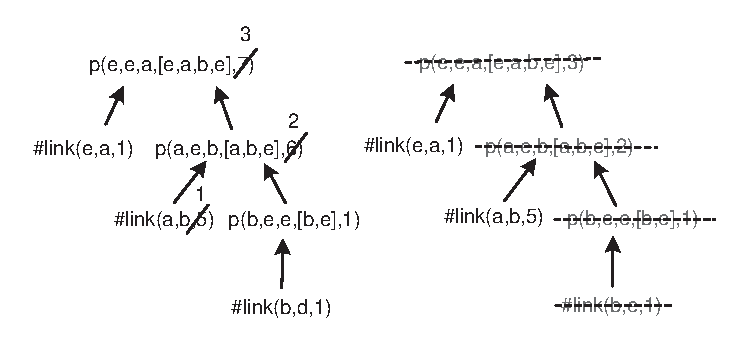
\epsfig{file=images/dtree.eps, width=3.5in}
\caption{\label{Derivation Tree}\emph{\small Derivation tree for derived
    path tuple from a to e. The left diagram shows updating the tree due
    to a change in base tuple $\#link({\bf a},b,5)$, and the right diagram shows
    the deletion of $\#link({\bf b},e,1)$.}}
\end{figure}                                              

%\footnote{In the case of BSN, on top of using
%  timestamps, we have to ensure that there are no two updates involving
%  tuples of the same primary key within a set that is being processed}.

%Let $t(0)$ denotes the initial value of tuple $t$, and $t(j)$ denotes the $j^{th}$ updated value of $t$.
%Let $tree(t)$ be the derivation tree (defined in Appendix~\ref{appendix:bursty}) for t with n leaf nodes,
%$l_{1}(0),l_{2}(0),...,l_{n}(0)$. Suppose each leaf has $u_{k}$ updates
%each. At the end of the updates, the $k^{th}$ leaf is
%$l_{k}(u_{k})$. Let $finalTree(t)$ be another derivation tree for t with n leaf nodes, where the $k^{th}$ leaf is
%initialize to $l'_{k}(0)=l_{k}(u_{k})$ for each of the leaf nodes. 
%The theorem means that for a given derivation tree whose leaf nodes are
%subjected to changes, if updates along any ``edge'' in the tree is
%applied in order, the eventual result at the root of the tree is based
%on the final state of the leaves. 

\subsection{Distributed Semantics}

In order for incremental evaluation to work in a distributed
  environment, it is essential that along any link in the network, there
  is a FIFO ordering of messages. That is, along any link literal \link(s,d), facts
  derived at node s should arrive at node d in the same order in which they
  are derived (and vice versa). This guarantees that updates can be
  applied in order. Using the same definition of $FP_{p}$ and $FFP_{p}$ as before, assuming the link FIFO ordering, in Appendix~\ref{appendix:burstyDistributed}, we prove the following
theorem:

\noindent{\bf Theorem ~\ref{theorem:netburst}: } {\em $FP_{p} = FFP_{p}$
in a distributed setting with FIFO links. }

%In fact, if we allow relax the link-restricted requirement of \Dlog and
%allow all nodes to communicate directly with each other, having the FIFO link ordering is not sufficient to
%guarantee eventual consistency.
The drawback of enforcing network link FIFO is that it increases the
  complexity and lowers the performance of the underlying network. The
  alternative adopted by network protocols is to maintain all tuples as
  {\em soft state}. In the soft state storage model, all data (base
  and derived tuples) has an explicit ``time to live'' (TTL), and
  facts (in our case base tuples) must be explicitly reinserted with
  their latest values and a new TTL or they are deleted. Reinsertion
  of base tuples
  leads to recomputation of query results, which in a quiescent
  network, leads to eventual consistency through the reinsertion of
  the facts from the quiescent state. 
  The drawbacks of soft state are well known:  recomputation can be expensive, and
  if done only periodically, the time to react to failures is a half-period on
  average.  However, soft state is often favored in networking
  implementations because in a very simple manner it provides eventually correct semantics in
  the face of reordered messages, node disconnection, and
  other unpredictable occurrences.\\


%\item {\bf Unique Derivation.} Each tuple sent as a message should have
%  a unique derivation. \Eg in the shortest-path query, all generated
%  $path$ tuples have a unique derivation (due the the path being
%  stored). This guarantees that we can differentiate tuples that are
%  derived along different paths in the network.


%\item {\bf Sender Address.} Each tuple that is
%  sent over the network during query execution must include the
%  immediate sender's address field at each hop.  \Eg in the
%  shortest-path query, all generated $path$ tuples include {\em nextHop}
%  field. The purpose of including this field is to allow
%  identical tuples that are derived along different paths to be
%  differentiated. This constraint can be checked by making sure all rule
%  heads include both address fields of the \link predicate.

%This requirement serves
%  two purposes. First, this allows tuples sent along different paths to
%  be differentiated. Second, this allows the deletion of facts
%  belongling to a neighbor whose link has been disconnected.
%  derived tuples that was previously sent by the neighbor. 
%This can be enforced on
%  all localized link-restricted rule heads by assigning the \link.@S
%  address field as one of the output attributes in the head.
%This is enforced on all
%  link-stricted rules that must include the locational specifier of the
%  body predicates.

%\end{mylist}
% the query, since derived tuples may need
%to be sent across the network, the FIFO ordering imposed by a local
%queue no longer holds, due to message reordering imposed by network
%delays and also losses. For example, it is conceivable that node {\em e}
% receives the older $path({\bf e},a,b,[e,a,c,d],3)$ before the newer path
% $path({\bf e},a,b,[e,a,c,d],2)$ due to reordering of
%  the $path$ tuples sent from node {\em a}, and hence computes the final
%  $shortestPath(e,b,[e,a,c,d],3)$ that does not reflect the latest state
%  of the network.



%\begin{figure}[ht]
%\centering
%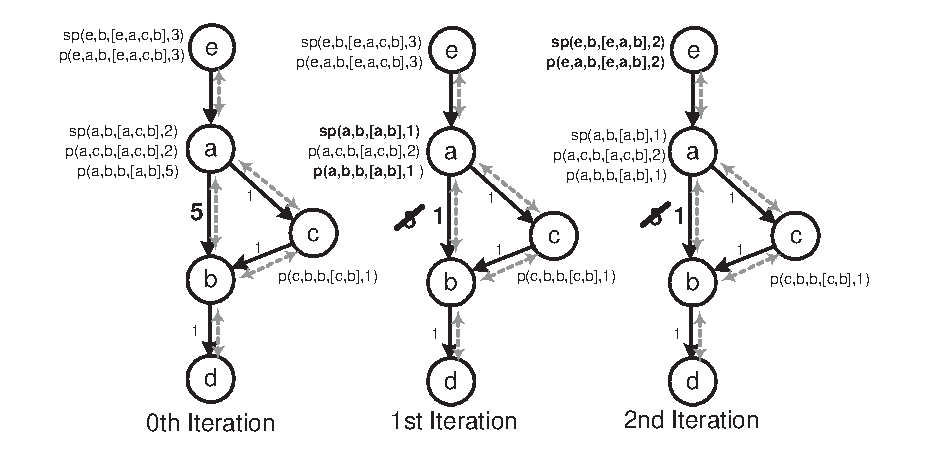
\epsfig{file=images/updateExample.eps, width=3.5in}
%\caption{\label{SP update example}\emph{\small All-Pairs Shortest Path Example
%    with update of link from $link({\bf a},b,5)$ to $link({\bf a},b,1)$. For
%    simplicity, we only show the computed paths and shortest paths to
%    destination node b. The derived tuples that are changed are
%    highlighted in {\em bold}.}}
%\end{figure}                                              

%Having shown incremental maintenance for the centralized case, we step
%through a distributed example, using the same derivation tree as
%before. We use the same network (Figure~\ref{SP update example})
%from our earlier query execution example in
%Section~\ref{sec:queryExec}. In the figure, at the $0^{th}$ iteration
%consists of the computed paths to destination node {\em b}. When
%$link({\bf a},b,5)$ is updated to $link({\bf a},b,1)$,
%$path({\bf a},-,c,[a,c],1)$ is updated at node {\em a}, and
%this results in the computation of $path({\bf e},a,[e,a,b],2)$ which is sent
%to node {\em e}. The shortest paths at each node are also updated
%accordingly to $shortestPath({\bf e},b,[a,b,],1)$ and
%$shortestPath({\bf e},b,[e,a,b],2)$ respectively.

% LocalWords:  recomputations fixpoint Bursty quiesces bursty FP PSN FFP BSN
% LocalWords:  recomputation nextHop stricted

\section{Query Optimizations}
\label{sec:queryOpt}
We proceed to discuss a set of query optimization opportunities
that arise in the declarative networking context.  These include
applications of traditional Datalog optimizations, as well as new
techniques for multi-query optimization, result caching, and
cost-based optimizations based on graph statistics. Some of these
techniques---in particular the use of traditional Datalog
optimizations and caching---were proposed in our previous
work~\cite{declareRoute}. We present extensions to our basic
techniques, as well as new avenues for optimization. 

Compared to the relatively solid foundation of the previous discussion,
 our approach here is more speculative: we open up a number of broad issues, and in
Section~\ref{sec:expr} we provide a taste of the potential benefits of
most of them via a full-fledged implementation running on a sizable
network testbed.  However our intention here is not to ``close the
book'' on any of these issues; much as in traditional database query
optimization and execution, we expect that our techniques here for
declarative networking will lead to significant work in a series of
more focused investigations.


\subsection{Traditional Datalog Optimizations}

We first explore the applicability of three traditional Datalog optimization
techniques: {\em aggregate selections}, {\em magic sets} and {\em
  predicate reordering}.

\subsubsection{Aggregate Selections}
\label{subsec:aggregateSelections}

A \naive execution of the {\em shortest-path} query computes all
  possible paths, even those paths that do not contribute to the eventual shortest
  paths. This inefficiency can be avoided with a query optimization
technique known as {\em aggregate selections}~\cite{sudarshan91aggregation,zaniolo}. 

Aggregate selections are useful when the running state of a monotonic
$AGG$ function can be used to prune query evaluation. For example, by applying
aggregate selections to the {\em shortest-path} query, each node only
needs to propagate the most current shortest paths for each destination
to neighbors. This propagation can be done whenever a shorter path is
derived.  

A potential problem with this approach is that the propagation of new
shortest paths may be unnecessarily aggressive, resulting in wasted communication.
As an enhancement, in the {\em periodic aggregate selections} scheme, a node buffers up
new paths received from neighbors, recomputes any new shortest paths
incrementally, and then propagates the new shortest paths
periodically. The periodic technique has the potential for reducing
network bandwidth consumption, at the expense of increasing convergence time.
It is useful for queries whose input tuples tend 
to arrive over the network out of order in terms of the monotonic aggregate --
\eg computing ``shortest'' paths for metrics that are  
not correlated with the network delays that dictate the arrival of the
tuples during execution.

In addition, aggregate selections are necessary for the termination of
some queries, as alluded to previously in
Section~\ref{sec:queryModel}. For example, with aggregate selections,
even if paths with cycles are permitted, the {\em
  shortest-path} query will terminate, avoiding cyclic paths of
  increasing lengths.  

%Example of queries that converges:
%\begin{itemize}
%\item Shortest path (C$_{1}+C_{2}$, min, C$>$0)
%\item Most reliable path (C$_{1}*C_{2}$, max, 0$\le$C$\le$1)
%\item Maximum capacity path (min(C$_{1},C_{2}$), max, C$>$0)
%\end{itemize}
%and Extension Tables~\cite{extension}. 

\subsubsection{Magic Sets and Predicate Reordering}
\label{sec:magic}
\label{sec:leftLinear}

The {\em shortest-path} query in our example computes {\em all-pairs} shortest
paths. This leads to unnecessary overhead when only a
subset of paths limited by sources and/or destinations is queried. This
problem can be alleviated by applying two optimization techniques:  {\em
  magic-sets rewriting} and {\em predicate reordering}.

\noindent
{\bf Magic-Sets Rewriting:} To limit query computation to the relevant portion
of the network, we use a query rewrite technique, called {\em
  magic sets rewriting}~\cite{oldMagic}. The Magic Sets method is
closely related to methods such as Alexander~\cite{alexander} and
QSQ~\cite{qsr}. Rather than review Magic Sets here,
we illustrate its use in an example: by modifying SP1 from the
shortest-path query, the following computes only paths limited to destinations
in the $magicDst$ table. 

\vspace{2pt}
{\small
\noindent{{\bf \#include(SP2,SP3,SP4)}} \\
\noindent{\bf SP1-D: } path({\bf @S},@D,@D,P,C) :- {\em magicDst({\bf
@D}),}\link{\em ({\bf @S},@D,C)},\\
\datalogspace P = $f\_concatPath$(link({\bf @S},@D,C), nil). \\
{\bf Query: } shortestPath({\bf @S},@D,P,C).
}
\vspace{2pt}


Rule SP1-D initializes 1-hop paths for destinations whose \\$magicDst({\bf @D})$
is present in the $magicDst$ table. This ensures that rule SP2 only
propagates paths to selected destinations based on the $magicDst$
table. The shortest paths are then computed as before using rules SP3
and SP4. 

\noindent
{\bf Predicate Reordering:} The use of magic sets in the previous query is not useful for pruning paths from
  sources. This is because paths are derived in a {\em ``Bottom-Up'' (BU)\/} fashion
  starting from destination nodes, where the derived paths are shipped
  ``backwards'' along neighbor links from destinations to sources. Interestingly, switching the search strategy
  can be done simply by {\em reordering} the $path$ and \link
  predicates. This has the effect of turning SP2 from a {\em right-recursive} to a {\em
  left-recursive} rule. Together with the use of magic sets, the
  following {\em magic-shortest-path} query allows filtering on {\em both} sources and {\em
  destinations}: 

\vspace{2pt}
{\small
\noindent{\bf SP1-SD: } pathDst({\bf @D},@S,@D,P,C) :- {\em magicSrc({\bf @S})}, \link({\bf @S},@D,C),\\
\datalogspace P = $f\_concatPath$(link({\bf @S},@D,C), nil). \\
{\bf SP2-SD: } pathDst({\bf @D},@S,@Z,P,C) :- {\em pathDst({\bf @Z},@S,@Z$_{1}$,P$_{1}$,C$_{1}$),}\\
\datalogspace\link({\bf @Z},@D,C$_{2}$), C := C$_{1}$ + C$_{2}$, \\
\datalogspace P = $f\_concatPath$(P$_{1}$,link({\bf @Z},@D,C$_{2}$)).\\
{\bf SP3-SD: } spCost({\bf @D},@S,min$<$C$>$) :- {\em magicDst({\bf
    @D})},\\
\datalogspace pathDst({\bf @D},@S,@Z,P,C).\\
{\bf SP4-SD: } shortestPath({\bf @D},@S,P,C) :- spCost({\bf @D},@S,C),\\
\datalogspace pathDst({\bf @D},@S,@Z,P,C).
%{\bf SP5-SD: } spResults({\bf @N},@S,@D,P,C) :- spResults({\bf
%  @N_{1},@S,@D,P,C),@N=f\_last(P),@N != null.
%{\bf SP6-SD: } shortestPath({\bf @S},@D,P,C) :- spResults({\bf @S},@S,@D,P,C).
}
\vspace{2pt}

The query computes 1-hop paths starting from each $magicSrc$
using rule SP1-SD. Rule SP2-SD then recursively computes new paths 
by following all reachable links, and stores these paths as
\texttt{pathDst( {\bf dst}, src, prevHop, pathVector, cost)} tuples at each
destination. Rules SP3-SD and SP4-SD then filter relevant paths based on $magicDst$, and compute the
shortest paths, which can then be propagated along the shortest paths back to the source node. In fact,
executing the query in this {\em ``Top-Down'' (TD)\/} fashion
resembles a network protocol called {\em dynamic source
routing}~\cite{dsr} which is proposed for ad-hoc wireless environments, where
the high rate of change in the network makes such targeted path
discovery more efficient compared to computing all-pairs shortest
paths. 


\subsection{Multi-Query Optimizations}
\label{subsec:multiQuerySharing}

In a distributed setting, it is likely that many related queries will be
concurrently executed independently by different nodes. A key requirement for scalability is the
ability to share common query computations (\eg pairwise shortest paths) among a potentially large number
of queries. We outline two basic strategies for multi-query sharing in
this environment: {\em query-result caching} and {\em
  opportunistic message sharing}. 


%\subsubsection{Query Results Caching}
%\label{subsec:magicCache}
\vspace*{.3em}\noindent
{\bf Query-Result Caching.\/}
Consider the {\em magic-shortest-path} query where node {\em a} computes
  $shortestPath({\bf a},d,[a,b,d],6)$ to node {\em d}. This cached value
  can be reused by all queries for destination {\em d} that pass
  through {\em a}, \eg the path from {\em e} to {\em d}. Currently, our implementation generates the cache internally, building a cache of all
the query results (in this case $shortestPath$ tuples) as they are sent
back on the reverse path to the source node. Since the subpaths of 
shortest paths are optimal, these can also be cached as an
enhancement. As ongoing work, we are exploring techniques for declaratively specifying
the cache, and evaluating caching policies. 
% To
%  utilize the cache, we can rewrite SP2-SD in the following way:%

%\noindent{\bf SP2-Cache: } spCacheHit({\bf @Z},@S,@D,P,C) :- {\em pathDst({\bf @Z},@S,@D,@Z$_{1}$,P$_{1}$,C$_{1}$),\\
%\datalogspace spCache({\bf @Z},@D,P$_{2}$,C$_{2}$)},  = C$_{1}$ + C$_{2}$, \\
%\datalogspace P = $f\_concatPath$(P$_{1}$,P$_{2}$).

%Rule SP2-Cache expresses the policy that the shortest path
%query for @S to @D can utilize the cache at node @Z if it
%exists. The generated $spCacheHit$ tuple is then sent back to the source
%node @S.




%\subsubsection{Opportunistic Message Sharing}
%\label{subsec:messageShare}
\vspace*{.3em}\noindent
{\bf Opportunistic Message Sharing.\/}
In the previous example, we consider how different nodes (src/dst) can
share their work in running the {\em same} query logic with different
constants. Sharing across {\em different} queries is a more difficult problem, since it
is non-trivial to detect query containment in
general~\cite{containment}. However, we observe that in many cases,
there can be correlation in the message patterns even for different
queries. One example arises when different queries request ``shortest'' paths based on different metrics, such as latency,
reliability and bandwidth; $path$ tuples being propagated for these
separate queries may be identical modulo the metric attribute being
optimized. 

A strategy that we have implemented is {\em opportunistic message
  sharing}, where multiple outgoing tuples that share common attribute
  values are essentially joined into one tuple if they are
  outbound to the same destination and share several common
  attributes; they can be re-partitioned at the receiving end. This
  achieves the effects of jointly rewriting the queries in a
  fashion, but on an opportunistic basis: derivations are
  done in this combined fashion only in cases that are
  spatiotemporally convenient during processing.
In order to improve the odds of achieving this sharing, outbound tuples
  may be buffered for a time and combined in batch before being sent.

As an alternative to this opportunistic sharing at the network level,
one can achieve explicit sharing at a logical level, \eg using correlated
aggregate selections for pruning different paths based on a combination
of metrics. For example, consider running two queries: one that computes
shortest latency paths, and another that computes max-bandwidth paths. We can
rewrite these as a single query by checking two aggregate selections,
\ie only prune paths that satisfy {\em both} aggregate
selections.



%\subsection{Hybrid Rewrites}
\subsection{Cost-Based Rewrites}
\label{subsec:hybridRewrites}

Currently, queries are executed using a left- (BU) or
right-recursive (TD) query expression (Section~\ref{sec:magic}).
Our main goal during query execution is {\em network efficiency\/} 
(\ie reducing the burden on the underlying network), which, typically,
also implies faster query convergence. 
It is not difficult to see that neither BU nor TD execution is universally 
superior under different network/query settings.
Even in the simple case of a shortest-path discovery query 
$shortestPath(@S,$ $@D,P,C)$ between two given nodes $(@S,@D)$,
minimizing message overhead implies that our query processor
should prefer a strategy that restricts execution to ``sparser'' regions
of the network (\eg \\doing a TD exploration from a sparsely-connected 
source $@S$).
%
%(Consider, for instance, the extreme case where $\calS=$ $\{s\}$ is only connected
%to a single chain of nodes leading to $\calD=$ $\{d\}$, whereas $d$ is a ``hub'' node
%with hundreds of neighbors.)
%In fact, as our discussion will show, in many scenarios, the optimal execution 
%strategy is a {\em hybrid search algorithm\/} that carefully combines both 
%BU and TD search.

We argue that {\em cost-based\/} query optimization techniques are needed 
to guarantee effective query execution plans.
While such techniques have long been studied in the context of relational 
database systems, optimizing distributed recursive queries for network
efficiency raises several novel challenges 
that we are exploring in our ongoing work.
In the remainder of this section, we briefly discuss some of our 
preliminary ideas in this area and their ties with work in 
network protocols.
%
%We essentially seek to optimize distributed recursive queries  for network efficiency
%over an asynchronous dataflow engine running on a given network topology; of course,
%adding additional problem characteristics (such as failure characteristics and network
%dynamics) only raises the complexity of the problem.

\vspace*{.3em}\noindent
{\bf The Neighborhood Function Statistic.\/}
As with traditional query optimization, cost-based techniques must
rely on appropriate {\em statistics\/} for the underlying execution
environment that can drive the optimizer's choices.
One such key statistic for network efficiency is the
{\em local neighborhood function\/} $N()$.
Formally, $N(X,r)$ is the number of distinct network nodes within
$r$ hops of node $X$.
The neighborhood function is a natural generalization of the size of the 
transitive closure (\ie reachability set) of a node, 
%%; furthermore, it is a
%fairly ``stable'' statistic (even though the specific nodes in the neighborhoods
%may change)  
that can be estimated locally (\eg through other recursive queries running in the background/periodically).
$N(X,r)$  can also be efficiently {\em approximated\/} through 
approximate-counting techniques using small (log-size) 
messages~\cite{anf}.
To see the relevance of $N()$ for our query-optimization problem, consider 
our example $shortestPath(@s,@d,P,$ $C)$ query,  and
let {\tt dist}($s,d$)  denote the distance of $s$, $d$ in the network.
A TD search would explore the network starting from node $s$, and 
% (assuming synchronous transmissions for simplicity)  
(modulo network batching) result in a total of
$N(s, {\tt dist}(s,d))$ messages  
(since it reaches all nodes within a radius of {\tt dist}($s,d$) from $s$). 
Note that each node only forwards the query message once, even though it may 
receive it along multiple paths.
Similarly, the cost for a BU query execution is $N(d, {\tt dist}(s,d))$.
%It is easy to see, 
However, neither of these strategies is necessarily
optimal in terms of message cost.
The optimal strategy is actually a {\em hybrid scheme\/} that ``splits'' the search 
radius dist($s,d$)
between $s$ and $d$ to minimize the overall messages; that is,
it first finds $r_s$ and $r_d$ such that:
%\begin{equation}
\vspace*{-6pt}\noindent
\[
(r_s, r_d)\ =\ \arg\min_{r_s+r_d = {\scriptsize\tt dist}(s,d)}\{\ N(s, r_s) + N(d, r_d)\ \},
%\label{eqn:singleopt}
%\end{equation}
\]
\vspace*{-10pt}\noindent
\noindent\\
and then runs concurrent TD and BU searches from nodes $s$ and $d$ (with radii $r_s$ and $r_d$,
respectively).
At the end of this process, both the TD and the BU search have intersected in 
at least one network node, which can easily assemble the shortest ($s,d$) path.
The above search strategy can be easily implemented as a rewrite
using simple \Dlog  rules.
While the above optimization problem is trivially solvable in
$O({\tt dist}(s,d))$ time, generalizing this hybrid-rewrite scheme
to the case of multiple sources and destinations raises difficult 
algorithmic challenges.
And, of course, adapting such cost-based  optimization algorithms
to work in the distributed, dynamic setting poses systems challenges.
Finally, note that neighborhood-function information can also 
provide a valuable indicator for the utility of a node as a result 
cache (Section~\ref{subsec:multiQuerySharing}) during query processing.
%(e.g. caches on ``hub'' nodes with rapidly-growing neighborhoods are more likely 
%to prove useful).



%%%%%%%%%%%%%%%%%%%%%%%%%%%%%%%%%%%%%%%%%%%%%%%%
\eat{
Now, while our hybrid-search optimization problem for the single shortest-path case 
(Equation~(\ref{eqn:singleopt})) is easily solvable (in $O({\mathrm dist}(s,d))$ time), 
the difficulty of the problem increases significantly when dealing with {\em multiple\/}
source and destination nodes.
Assume that we want to discover shortest paths between all sources 
$\calS=$ $\{s_1,$ $\ldots,$ $s_m\}$ and all destinations
$\calD=$ $\{d_1,$ $\ldots,$ $d_n\}$; then, a message-optimal hybrid-search strategy 
must use an $m$-tuple of source radii $(r_{s_1},$ $\ldots,$ $r_{s_m}\}$ that 
minimize the expression
\begin{equation*}
\sum_i N(s_i, r_{s_i})\ +\ \sum_j N(d_j, \max_i\{ {\mathrm dist}(s_i, d_j)-r_{s_i} \})
\end{equation*}
where the $\max\{\}$ term in the second sum ensures that the search neighborhoods
intersect {\em for all\/} $(s_i, d_j)$ pairs.
The complexity of obvious solutions to the above problem explodes exponentially in $m$,
and we are currently working on more efficient optimization strategies.

Of course, the above discussion assumes an ideal, ``centralized'' problem setting,
where the optimizer has access to the the distance and neighborhood-function 
information for all nodes involved in the query.
Adapting such cost-based optimizations to a distributed setting raises additional
challenges.
One possible solution is to maintain repository-nodes inside the network where 
the optimizer can access relevant distance and neighborhood-function 
statistics.
Another option is to allow nodes to employ more sophisticated, incremental 
path-discovery algorithms (\eg based on {\em expanding-ring search}~\cite{expring})
driven by their local neighborhood-function information.
We are exploring these options in the next-generation algorithms.

%
%One area of optimizations we are exploring is on the use of a
%hybrid strategy, where queries are computed using a mixture of both
%strategies. {\em MINOS's}

}
%%%%%%%%%%%%%%%%%%%%%%%%%%%%%%%%%%%%%%%%%%%%%%%%


\vspace*{.3em}\noindent
{\bf Adaptive Network Routing Protocols.\/}
While we do not evaluate the above concepts in our experiments below,
we note that the networking literature has considered adaptive routing protocols
that strongly resemble our use of hybrid rewrites; hence, we believe
this is an important area for future investigation and generalization.
One interesting example is the class of
{\em Zone-Routing Protocols} (ZRP)~\cite{zrp}.
A ZRP algorithm works by each node precomputing {\em k-hop-radius\/} shortest paths to
neighboring nodes (in its ``zone'')  using a BU strategy.
Then, a shortest-path route from a source to destination is computed in a
TD fashion, using essentially the {\em magic-shortest-path} query described above, 
utilizing any precomputed shortest paths along the way.
Each node sets its zone radius $k$ adaptively based on the density and rate of change of 
links in its neighborhood; in fact,
recent work~\cite{sharp} on adjusting the zone radius for ZRP-like routing uses
exactly the neighborhood-function statistic.
% discussed earlier in this
%section. 



%\subsection{Gossip-Based Approximations}
%OPTIONAL if time permits.
%When receive paths, compute new paths based on subset of links. Simple
%change in rules, add a f\_coinFlip predicate to rules for computing links.






%\subsection{Query Approximations}
%Suppress best path messages that are within X\% of last advertised. For
%example, if we are willing to tolerate X\% errors of each path, then
%each node only needs to send path messages to neighboring nodes if the
%current path improves upon previous by $>$X\%. The actual worst-case margin of
%error is closer to $1-((1-X)^k)$, where k is the hop count diameter of the network.

%Another form of approximation applies to multi-objective queries, for
%example all-pairs best paths queries that optimizes for both latency and
%loss-rates. Skylines can be used to compute the dominating paths along
%multiple metric dimensions, but are expensive when objectives are not highly correlated. We can make
%use of approximate skylines in this case. 
%\subsection{Multi-Objective Queries}
%Optional. Skylines and approximate skylines. Skylines are expensive
%unless the multiple objectives are highly correlated.



\begin{figure*}[ht]
	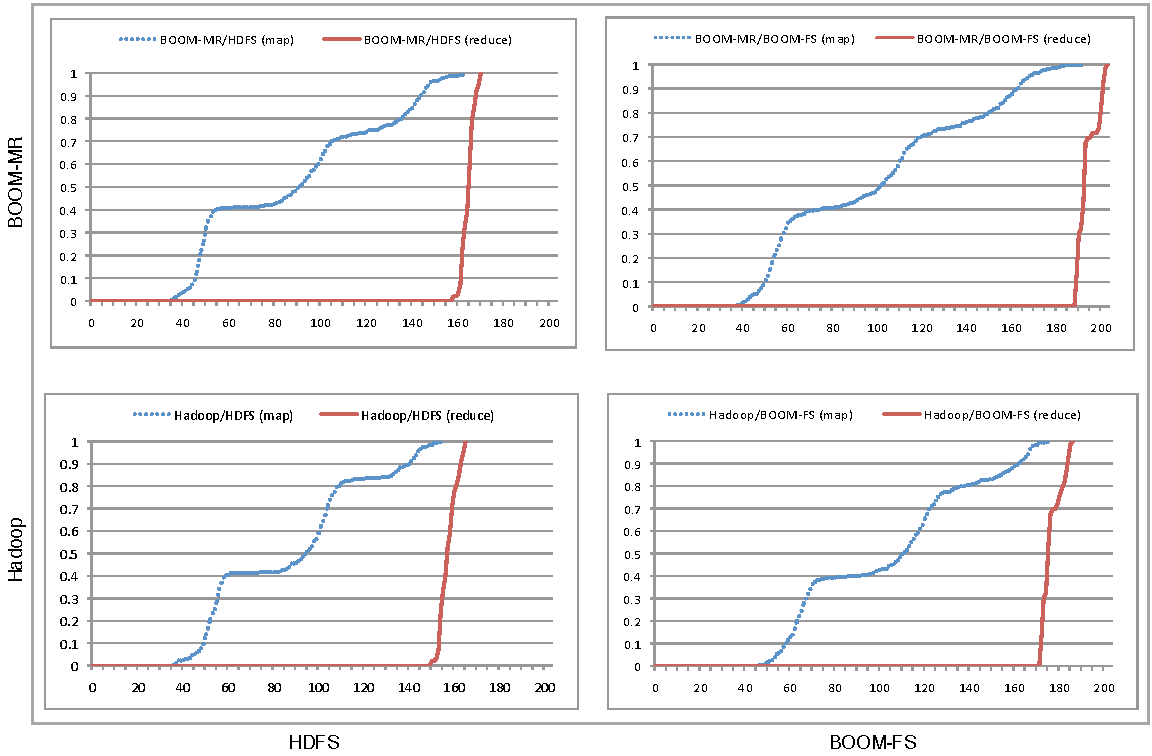
\includegraphics[width=0.95\linewidth]{graphs/fourgraphs}
% \begin{minipage}{0.5\linewidth}
%         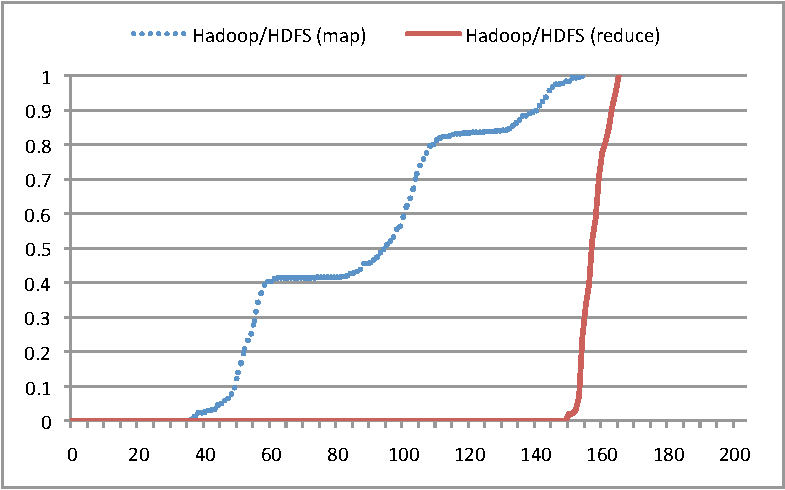
\includegraphics[width=0.95\linewidth]{graphs/hadoop_hdfs}
% \end{minipage}
% \begin{minipage}{0.5\linewidth}
%         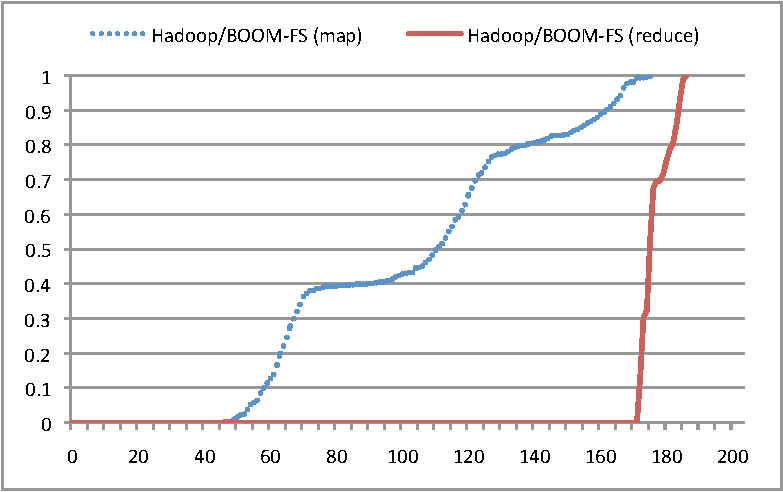
\includegraphics[width=0.95\linewidth]{graphs/hadoop_bfs}
% \end{minipage}
% \begin{minipage}{0.5\linewidth}
%         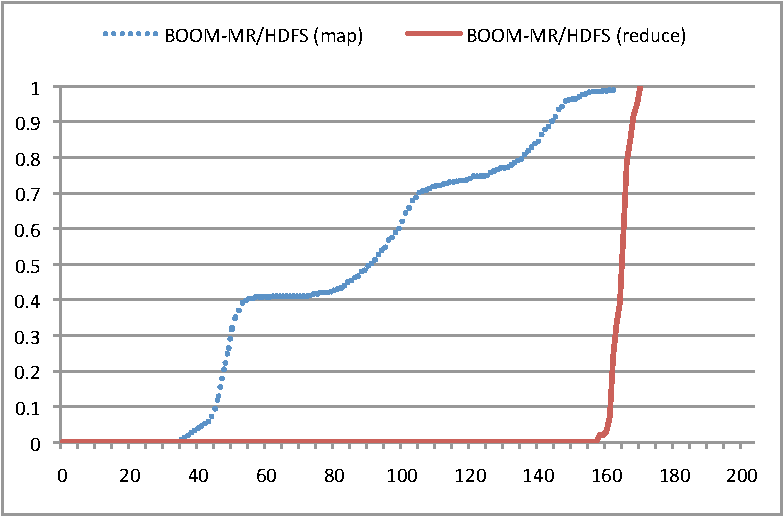
\includegraphics[width=0.95\linewidth]{graphs/bmr_hdfs}
% \end{minipage}
% \begin{minipage}{0.5\linewidth}
%         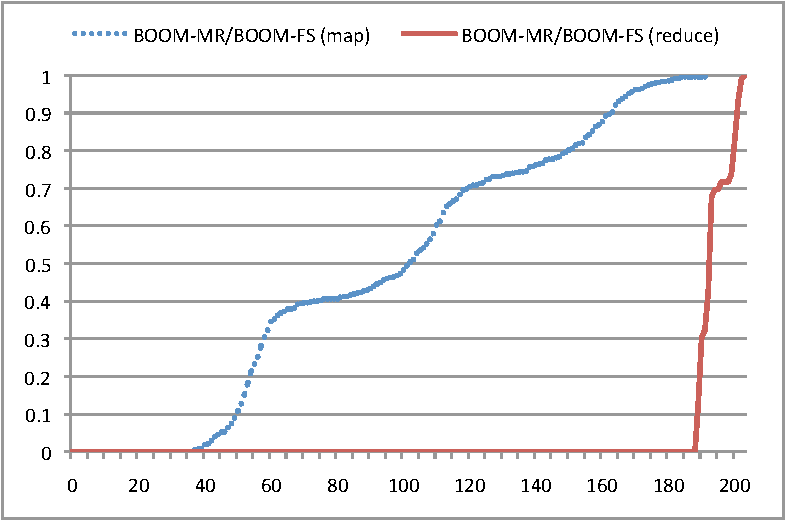
\includegraphics[width=0.95\linewidth]{graphs/bmr_bfs}
% \end{minipage}
\caption{CDFs representing the elapsed time between job startup and task
  completion for both map and reduce tasks, for all combinations of Hadoop and \BOOM-MR
  over HDFS and \BOOM-FS\@.  In each graph, the horizontal axis is
  elapsed time in seconds, and the vertical represents the percentage of tasks completed.}
\label{fig:ec2experiment}
\vspace{-8pt}
\end{figure*}

\section{Performance Validation}
\label{sec:eval}
While improved performance was not a goal of our work, we wanted to
ensure that the performance of \BOOMA was competitive with Hadoop.
We compared \BOOMA with Hadoop 18.1, using the 101-node EC2 cluster
described in Section~\ref{sec:schedeval}. The workload was a wordcount job
on a 30 GB file, using 481 map tasks and 100 reduce tasks.

Figure~\ref{fig:ec2experiment} contains four graphs comparing the performance of
different combinations of Hadoop MapReduce, HDFS, \BOOM-MR, and \BOOM-FS\@. Each
graph reports a cumulative distribution of the elapsed time in seconds from job
startup to map or reduce task completion. The map tasks complete in three
distinct ``waves.'' This is because only 2 $\times$ 100 map tasks can be
scheduled at once. Although all 100 reduce tasks can be scheduled immediately,
no reduce task can finish until all maps have been completed because each reduce
task requires the output of all map tasks.

The lower-left graph describes the performance of Hadoop running on top of HDFS,
and hence serves as a baseline for the subsequent graphs. The upper-left graph
details \BOOM-MR running over HDFS\@. This graph shows that map and reduce task
durations under \BOOM-MR are nearly identical to Hadoop 18.1. The lower-right
and upper-right graphs detail the performance of Hadoop MapReduce and \BOOM-MR
running on top of \BOOM-FS, respectively. \BOOM-FS performance is slightly
slower than HDFS, but remains competitive.

% The LATE policy presents an alternative scheme for speculative task
% execution on {\em straggler} tasks~\cite{late-sched}, in an effort to
% improve on Hadoop's policy.  There are two aspects to each policy:
% choosing which tasks to speculatively re-execute, and choosing {\TT}s
% to run those tasks.  Original Hadoop re-executes a task if its
% progress is more than 0.2 (on a scale of $[0..1]$) below the mean
% progress of similar tasks; it assigns speculative tasks using the same
% policy as it uses for initial tasks. LATE chooses tasks to re-execute
% via an {\em estimated finish time} metric based on the task's
% \emph{progress rate}. Moreover, it avoids assigning speculative tasks
% to {\TT}s that exhibit slow performance executing similar tasks, in
% hopes of preventing the creation of new stragglers.

%%The LATE policy is specified in the paper via just three lines of
%%pseudocode, which make use of three performance statistics called {\em
%%  SlowNodeThreshold}, {\em SlowTaskThreshold}, and {\em
%%  SpeculativeCap}.  The first two of these statistics correspond to
%%the 25th percentiles of progress rates across {\TT}s and across tasks,
%%respectively.  The {\em SpeculativeCap} is suggested to be set at 10\%
%%of available task slots~\cite{late-sched}.  We compute these
%%thresholds via the five Overlog rules shown in
%%Figure~\ref{fig:latePolicy}.  Integrating the rules into \BOOM-MR
%%required modifying two additional Overlog rules that identify tasks to
%%speculatively re-execute, and that choose {\TT}s for scheduling those
%%tasks.

% If a \TT asks for new a new task and there are fewer than {\em SpeculativeCap} speculative tasks running:
% \begin{enumerate}
% \item Ignore the request if the \TT progress for running tasks is below some {\em SlowNodeThreshold}
% \item Rank current running tasks by the estimated finish time
% \item Launch a copy of the highest-ranked task with progress rate below {\em SlowTaskThreshold}
% \end{enumerate}


%The primary inputs to the LATE policy are the {\em SpeculativeCap}, {\em SlowTaskThreshold} and the {\em SlowNodeThreshold} values, which provide thresholds for pruning tasks and nodes from consideration. The SpeculativeCap is a single system level query maintained in the scheduler.olg module, and is used to limit the total number of speculative map and reduce tasks. SlowTaskThreshold and SlowNodeThreshold values are categorized by the job identifier and task type (map or reduce). Selecting which tasks to speculate, and on which trackers they should execute, required changes to two queries in the first-come first-serve policy.olg module and the additional 6 queries. %shown in  Figure~\ref{fig:latePolicy}. 

%A task is only considered for speculation if its progress rate falls below the SlowTaskThreshold in its given category.  Queries L1 - L3 maintain this threshold value for each category. Query L1 determines the progress rate for a given task based on its current progress and running time. Query L2 forms a list of the progress rates for each task category. Finally, query L3 computes a SlowTaskThreshold for each task type of a job by taking the lower 25th percentile of the progress rate list. 
%The LATE policy ensures that speculative tasks execute on ``fast'' nodes by pruning \TT nodes whose rate of progress for a given task category fall below some threshold. Queries L4 - L6 maintain this threshold value for each task category. The first query L4, computes the average progress that a given \TT has made for each task category and stores that result in the taskPR table. Query L5 forms a list of the average progress rates out of each category by aggregating over the taskPR table, and the result of this query is stored in the trackerPRList table. Query L6 computes the slowNodeThreshold for each category by taking the 25th percentile of the list of rates stored in the trackerPRList table.


% \jmh{Tyson/Khaled to write one paragraph here on the size/complexity of the LATE implementation.}
% 
% \jmh{Tyson/Khaled to write on paragraph here with motivation for
% affinity scheduler here, a sketch of the policy that was
% implemented.}

% \subsection{LATE Evaluation}
% Figure~\ref{fig:ec2reduce} shows the cumulative distribution of the
% completion time for reduce task executions on EC2 under normal load,
% and with artificial extra load placed on six straggler nodes.  The
% same wordcount workload was used for this experiment but the number of
% reduce tasks was increased from $100$ to $400$ in order to produce two
% waves of reduce tasks.  The plots labeled ``No Stragglers'' represent
% normal load.  The plots labeled ``Stragglers'' and ``Stragglers
% (LATE)'' are taken under the (six node) artificial load using the
% vanilla Hadoop and LATE policies (respectively) to identify
% speculative tasks.  We do not show a CDF of the map task execution
% time since the artificial load barely affects it --- the six
% stragglers have no effect on other map tasks, they just result in a
% slower growth from just below $100\%$ to completion.
% %Figure~\ref{fig:ec2map} shows that the delay due to the loaded map stragglers only
% %affects those six nodes.  
% The first wave of $200$ reduce tasks is scheduled concurrently with
% all the map tasks. This first wave of reduce tasks will not finish
% until all map tasks have completed, which increases the completion time
% of these tasks as indicated in the right portion of the graph. The
% second wave of $200$ reduce tasks will not experience the delay due to
% unfinished map work since it is scheduled after all map tasks have
% finished. These shorter completion times are reported in the left
% portion of the graph. Furthermore, stragglers have less of an impact
% on the second wave of reduce tasks since less work (i.e., no map work)
% is being performed. Figure~\ref{fig:ec2reduce} shows this effect, and
% also demonstrates how the LATE implementation in \BOOMA handles
% stragglers much more effectively than the default speculation policy
% ported from Hadoop.  This echoes the results of Zaharia et
% al.~\cite{late-sched}



\section{Additional Related Work}
We mentioned most of the related work in the context of our discussion
above.  Here, we briefly mention some other related efforts.

% Optimization and execution of recursive queries is a rich area of
% research; Ramakrishnan and Ullman's survey~\cite{ramakrishnan93survey}
% provides a variety of references to the literature.  

We are not alone in our renewed enthusiasm for applications of
recursive queries.  There are other contemporary examples from outside the
traditional database ``market'', including software
analysis~\cite{whaley04}, trust management~\cite{Cassandra} and
diagnosis of distributed systems~\cite{discreteEventDatalog}.  Our
concept of {\em link-restricted} rules is similar in spirit to {\em
  d3log}~\cite{jimsuciu}, a query language based on Datalog proposed
for dynamic site discovery along web topologies.

Much research in the
parallel execution of recursive queries~\cite{cacace93survey} has
focused on high throughput within a cluster. In contrast, our
strategies and optimizations are geared towards bandwidth efficiency
and fast convergence in a distributed setting.  Instead of hash-based
partitioning schemes that assume full connectivity among nodes, we are
required to perform query execution only along physical network links
and deal with network changes during query execution.  There is also
previous empirical work on the performance of parallel pipelined
execution of recursive queries~\cite{pipelinedRecursive}. Our results
extend that work by providing new, provably correct pipelining
variants of semi-\naive evaluation.

In terms of distributed systems, the closest analog is the recent work
by Abiteboul \textit{et al.}~\cite{discreteEventDatalog}.  They adapt
the QSQ~\cite{qsr} technique to a distributed domain in order to
diagnose distributed systems.  An important limitation of their
approach is that they do not consider partitioning of relations across
sites as we do; they assume each relation is stored in its entirety in
one network location. Further, they assume full connectivity and do not
consider updates concurrent with query processing.


%There are proposals for instantiating networking protocols
%from high-level specifications from the formal methods community.
%For example,~\cite{maude} applies Maude, an executable specification
%language based on rewriting logic to the field of network security
%protocols.  Within the traditional networking, there is also renewed
%interest in high-level specification.  For example,
%Metarouting~\cite{metarouting} deals with ``routing algebras'' which
%specify routing protocol behavior globally.  We are investigating
%implementing Metarouting over \Sys and \Dlog. 

% Apart from declarative networks, there have been other recent proposals
% on interesting applications of Datalog and recursive queries outside of traditional data
% management domains. Abiteboul \textit{et~al.}~\
% \cite{discreteEventDatalog}  demonstrate how the diagnosis of distributed systems
% can be modeled using Datalog programs, and can benefit from optimization
% techniques such as Query-Sub-Query (QSQ)~\cite{qsr}, which is related to
% our use of the magic sets optimizations. It has also been shown that
% many program analysis can be expressed naturally and easily in logic
% programming languages~\cite{logicProgramAnalysis}. In a recent work, Whaley \textit{et~al.}~\ \cite{whaley04} demonstrated the advantages (in terms of programmability and
% performance) of having a declarative interface for pointer analysis of
% large programs.  

\section{Conclusion}
\label{sec:conclusion}
\label{sec:futurework}

Our goal in this paper was twofold: to provide a solid database
foundation for recent developments in declarative networking, and to
open a number of database research directions in the area.  We believe
that our contributions here are significant on both fronts.

We started with the concept of \emph{link-restricted rules}, which
capture syntactically in \Dlog the notion that query
messages are constrained to travel along direct links between nodes in
a network.   This in turn led to successive refinements of
semi-\naive evaluation that deal efficiently
with the asynchrony and delays intrinsic to a wide-area networking
environment.  We introduced techniques to incorporate updates
immediately during execution, capturing the reactive nature of
typical network protocols while offering meaningful semantic
guarantees.  We  also discussed a number of
query optimization techniques, and their applicability to the networking
domain.  Finally, we presented evaluation results from a distributed deployment
  involving 100 machines on the Emulab~\cite{emulab} network testbed, running prototypes of our optimization techniques implemented as
  modifications to the \Pitu system.  

%the
%adaptation of cost-based magic-sets~\cite{costMagic} for
%the distributed setting, 

%Declarative networking is a promising area with some interesting
%challenges for database researchers.  
Our ongoing research is proceeding in several directions. First, we are
exploring a complete query optimization architecture, as well as
specific techniques beyond those of
Section~\ref{sec:queryOpt}: additions to the cost-based
optimizations of Section~\ref{subsec:hybridRewrites}
including the possibility of using random walks driven by statistics
on graph expansion; adaptive query processing techniques to react to
network dynamism; and multi-query optimizations motivated by more
complex overlay networks. Second, we plan to incorporate
negation into our model and implementation~\cite{ullmanNegation},
which raises interesting challenges
for pipelining and dynamic data. Third, a key selling point of
declarative languages in the networking community is the promise of
static program checks for desirable network protocol properties;
% such as convergence and stability; 
we are considering techniques from the
Datalog literature in this regard (\eg ~\cite{krs}) and expect that
the particulars of link-restricted rules can be of use as well.
Finally, we intend to aggressively pursue these ideas in the context of
serious networking applications, \eg overlay networks like distributed hash
tables, application-level multicast protocols, and virtual private networks.

%Second, we will revisit some of \Dlog's restrictions, in particular
%link-restricted rules for specifying more complex networks. So far our programs
%have performed global recursive computations along network links; we
%wish to study more execution semantics in the presence of locally
%recursive rules. 

We have been pleased in this work to see that the enthusiasm in the
networking community for declarative languages can provide more than
just a well-motivated application area for recursive queries; it
appears to spark a host of new database research challenges in what
was considered a very mature area.  We are optimistic about the
potential for additional significant results in this domain, in terms
both of theoretical work and systems challenges.

%% Use the next sentence of Stonebraker's quote in the intro, which is:
%% ``If a market develops for [recursive query] technology, the
%% commercial DBMSs will implement the ideas in a heartbeat.''  Well,
%% maybe not Oracle, but maybe Cisco instead!


%However, even with stratified negation, determining the right pipelining strategy in the asynchronous
%  distributed setting is a challenge. 
%Just as we relax the need to
%  perform semi-\naive evaluations in iteration, we intend to explore the relaxation
%  of evaluating programs with negation a stratum at a time, where evaluation results can be
%  corrected over time with updates, leading to eventual consistency.

%\end{mylist}



%\linespread{0.95}
{\scriptsize
\bibliographystyle{abbrv}
\bibliography{biblio}
}

\subsection{Stratification in {\large{\bf\slang}}}
\label{sec:strat}
We first turn our attention to the semantics of
programs with negation.  As we will see, the inclusion of time enables
programs' local stratification, and the existence of a unique perfect model
that corresponds to intuition. \wrm{reword}

%``source of monotonicity''  a unique perfect model

%semantics in some surprising cases, and enables purely syntactic monotonicity
%checks for a broad class of temporal programs.

%%\paa{notes}

%%this section has become cluttered, but for me the main results are the following:

%%\begin{enumerate}
%%\item Negation-, aggregation- and choice-free \lang programs have a unique minimal model (pure Datalog)
%%\item stratifiable \lang programs have a unique minimal model (again, Datalog, but we need to show that the restrictions and syntactic transformations
%%cannot introduce a cycle or add a negative edge to an existing cycle.)
%%\item \emph{temporally stratified} \lang programs (w/o choice) force any cycles with negation to involve an inductive edge, forcing an ordering on the evaluation.
%%we can show that in all such cases, the corresponding datalog program is modularly stratified (insofar as \emph{successor} is considered to be ``completely
%%evaluated" in a lower module.)  since modularly stratified programs have a unique stable model, so do any temporally stratified \lang programs.
%%\end{enumerate}

\begin{lemma} \label{lemma:no-neg-unique}
%
A \slang program without negation 
%%and aggregation 
has a unique minimal model.
%
\end{lemma}

\begin{proof} 
%
A \slang program without negation 
%%and aggregation 
is a pure Datalog
program.  Every pure Datalog program has a unique minimal model. 
%
\end{proof}

%%\jmh{Oops, you forgot that this model is countably infinite due to infinite time. So I could add countably many random consistent facts and have an equally ``small'' model. You will need a more refined definition of safety and minimality that accounts for time.}

%%\jmh{I'm going to stop commenting here since you'll need some more machinery to continue.}

We define syntactic stratification of a \slang program the same way it is
defined for a Datalog program:

\begin{definition}
%
A \slang program is \emph{syntactically stratifiable} if there
exists no cycle with a negative edge 
%%or an aggregation edge 
in the program's
predicate dependency graph.
%
\end{definition}

%%We evaluate such a program by evaluating each strongly connected component of
%%its predicate dependency graph under a closed-world assumption.  

We may evaluate such a program in {\em stratum order} as described in the
Datalog literature~\cite{ullmanbook}.
%%\wrm{cite?}
%any order returned by a topological sort on the predicate dependency graph,
%with each strongly connected component collapsed to a single node.
It is easy to see that any syntactically stratified \slang instance has a
unique perfect model \wrm{cite?} because it is a syntactically stratified Datalog program.

%\begin{lemma}
%
%A syntactically stratifiable \lang instance without choice has a unique
%minimal model.  That is, there exists a function $D$ from syntactically
%stratifiable \lang instances without choice to their minimal models.
%
%\end{lemma}

%\begin{proof}
%\wrm{todo: insert statement that this is obvious}
%
%We know that there exists a function $B$ from syntactically stratifiable
%Datalog instances to their minimal models \wrm{cite?}.  Earlier, we introduced
%\wrm{XXX: where?} a bijection \wrm{XXX: probably not a bijection} $A$ from the
%set of \lang instances without choice to the set of Datalog instances, and a
%bijection $C$ between minimal models of Datalog instances and minimal models of
%\lang instances without choice.  We will show that $D = C \circ B \circ A$.

%Thus, we need only prove that the restriction of $A$ to syntactically
%stratifiable \lang instances without choice maps to a subset of syntactically
%stratifiable Datalog instances.  But this is clear, as $A$ does not add any
%rules to the instance, and may introduce only the non-negated EDB {\em
%successor} relation to the body of an existing rule.  Thus, $A$ cannot
%introduce any new cycle or add negation to any existing cycle in the instance's
%predicate dependency graph.
%
%\end{proof}

However, many programs we are interested in expressing are not syntactically
stratifiable.  Fortunately, we are able to define a syntactically checkable
notion of {\em temporal stratifiability} of \slang programs that maps to a
subset of {\em locally stratifiable} \wrm{cite, and mention this term was coined previously} Datalog programs.

%Intuitively, a Datalog instance is modularly stratifiable if no EDB
%element depends negatively on itself.

%%\begin{example}
%%Consider a predicate \emph{print} that corresponds to a print queue.  The program below
%%states that if there is a message \{A, B\}, then there 
%%\begin{Dedalus}
%%print(A, B) \(\leftarrow\)
%%  message(A, B),
%%  \(\lnot\)print(A, B);
%%\end{Dedalus}
%%\end{example}

%Peter said we might not need these formal definitions.  Experimenting without
%\begin{definition}
%
%A Datalog program and EDB is \emph{locally stratifiable} if, after
%instantiating the rules given the Herbrand saturation of the program and EDB,
%there exists no cycle with a negation or aggregation edge in the dependency
%graph of instantiated ground atoms.
%
%\end{definition}

%We take the definition below from Ross~\cite{modular, ross-syntactic}.
%\begin{definition}
%
%A Datalog instance is \emph{modularly stratifiable} if, and only if its
%mutally recursive components are locally stratified once all instantiated rules
%with a false subgoal that is defined in a ``lower" component are removed.
%\end{definition}

%\begin{lemma}
%
%A locally stratifiable \lang instance without choice has a unique
%minimal model.  That is, there exists a function $E$ from locally
%stratifiable \lang instances without choice to their minimal models.
%
%\end{lemma}

%\begin{proof}
%
%\wrm{TODO}
%
%\end{proof}


\begin{definition} 
%
The \emph{deductive reduction} of a \slang program $P$ is
the subset of $P$ consisting of exactly the deductive rules in $P$.
%
\end{definition}

\begin{definition} 
%
A \slang program is \emph{temporally stratifiable} if its deductive
reduction is syntactically stratifiable.
%
\end{definition}

\wrm{major false depth here, I say we eliminate the theorem and just cite
Datalog/UT here: ``This paper has shown that by making the local stratification
of programs explicit in time stamps a pure logical theory of updates is
possible.''}

%%\newtheorem{theorem}{Theorem}
\begin{lemma}
\label{lemma:temp-strat-uniq}
%
Any temporally stratifiable \slang instance $P$ has a unique perfect model.
%
\end{lemma} 

\begin{proof}
%
{\bf Case 1:} $P$ consists of only deductive rules.  In this case, $P$'s
deductive reduction is $P$ itself.  We know $P$ is syntactically stratifiable,
thus it has a unique perfect model.

{\bf Case 2:} $P$ consists of both deductive and inductive rules.  Assume that
$P$ does not have a unique perfect model.  \wrm{and the proof requires a bit of
touching up here...}

This implies that $P$ is not
syntactically stratifiable.  Thus, there must exist some cycle through at least
one predicate $q$ involving negation.
%%or aggregation.  
Furthermore, this cycle must involve an inductive rule, as $P$ is temporally
stratified.

Since the time suffix in the head of an inductive rule is strictly greater than
the time suffix of its body, no atom may depend negatively on itself---it may
only depend negatively on atoms in the previous timestep.  Thus, $P'$ is
{\em universally contraint stratified} because induction through time implies a
monotonicity constraint \wrm{cite Ross}.  This guarantees a unique perfect model
achievable via standard bottom-up fixpoint execution.
%
%does not have a unique minimal model.  This implies that $P$ is not
%syntactically stratifiable, thus there must exist some cycle through at least
%one predicate $q$ involving a negation or aggregation edge in $P$'s predicate
%dependency graph, and furthermore this cycle must include at least one
%inductive rule.  Since an inductive rule has a time suffix $S := N+1$, where
%$N$ is the timestamp of its body, and $P$'s deductive reduction is
%syntactically stratifiable, we know that the aggregate or negation of $q$ must
%always occur in a strictly earlier or later timestamp than that of the
%positive $q$ atom.  Since the timestep in the cycle increases monotonically
%with each iteration, $q$ will never, in practice, depend on a negation or
%aggregate of itself.  Thus, $P$ is locally stratifiable, and by Lemma XXX
%above, $P$ has a unique minimal model.  This contradicts our assumption that
%$P$ does not have a unique minimal model.  Thus, $P$ has a unique minimal
%model.
%
\end{proof}


\begin{example}
A simple temporally stratifiable \slang program that is not syntactically stratifiable.

\begin{Dedalus}
persist[p, p\_neg, 3]  
  
r1
p(A, B, T) \(\leftarrow\)
  insert\_p(A, B, T);

r2  
p_neg(A, B, T) \(\leftarrow\)
  p(A, B, T),
  delete\_p(T);
\end{Dedalus}

In the \slang program above, \emph{insert\_p} and \emph{delete\_p} are captured
in EDB relations.  This reasonable program is unstratifiable because $p \succ
p\nega \land p\nega \succ p$.  But because the successor relation is
constrained such that $\forall A,B, successor(A, B) \rightarrow B > A$, any
such program is locally stratified on time suffixes.  Therefore, we have
$p_{n} \not\succ^* p\_neg_{n} \not\succ^* p_{n+1}$; informally, earlier values
do not depend on later values.
%%\paa{need to make the text better, but this old example probably makes sense here}
\end{example}

\begin{figure}[t]
  \centering
  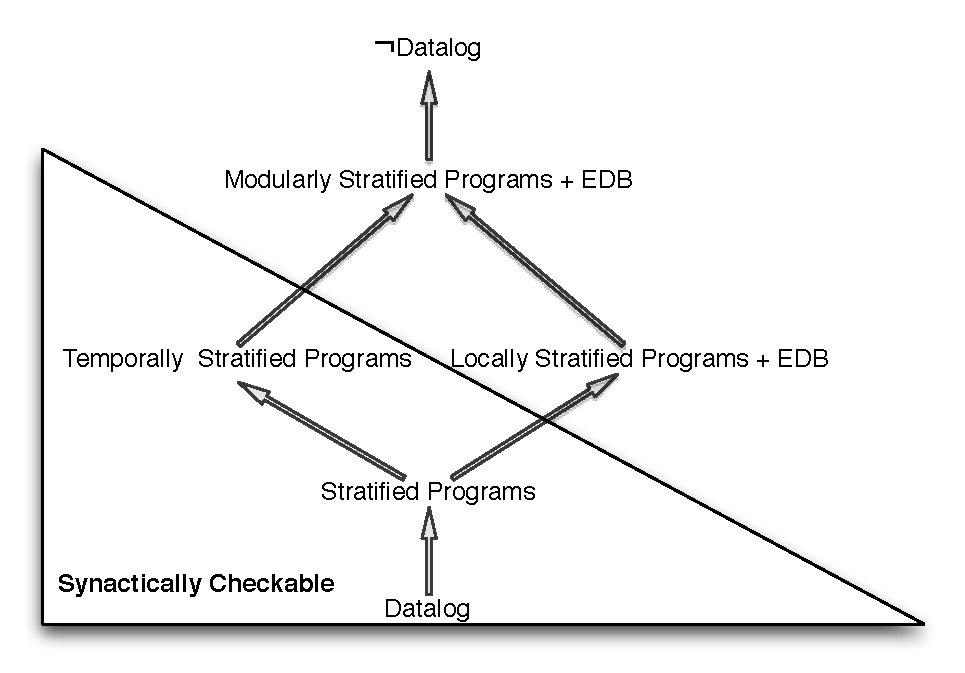
\includegraphics[width=0.75\linewidth]{figures/dedalus_classes.pdf}
  \label{fig:dedalus-classes}
  \caption{Stratifiability classes.  $A \to B$ means that every program in $A$ is in $B$.}
\vspace{-8pt}
\end{figure}


%%\paa{I don't think we can show that programs with async rules are locally stratifiable, actually}
%%\wrm{Why not?  What if we have that "causality constraint" we were talking about?}


\end{document}
